% This is samplepaper.tex, a sample chapter demonstrating the
% LLNCS macro package for Springer Computer Science proceedings;
% Version 2.20 of 2017/10/04
%
\documentclass[12pt, a4paper]{article}

\usepackage[russian]{babel}
\usepackage{graphicx}
% Used for displaying a sample figure. If possible, figure files should
% be included in EPS format.
%
% If you use the hyperref package, please uncomment the following line
% to display URLs in blue roman font according to Springer's eBook style:
% \renewcommand\UrlFont{\color{blue}\rmfamily}
\usepackage{amssymb}
\usepackage{amsbsy}

\usepackage{xcolor}

\newcommand{\bs}{\boldsymbol}

\begin{document}

\begin{center}
{\bf Analysis of $MAP/G/1$ queue with inventory as the model of the node of wireless sensor network with energy harvesting}
\end{center}

\begin{abstract}
Queueing systems where certain inventory items are required to provide service to a customer become popular in the literature. Such systems are similar to the analysed in the literature models with paired customers, assembly-like queues, passenger-taxi models, etc. During the last few years they are considered in context of  modelling operation of the nodes of a wireless sensor network with energy harvesting.  Distinguishing feature of the model considered in this paper, besides the suggestion that arrival flow of customers is described by the Markovian Arrival Process,  is the assumption about a general distribution of the service time while only exponential or phase-type distribution was previously assumed in the existing literature. We apply the well-known technique of $M/G/1$ type Markov chains and semi-regenerative processes to obtain the ergodicity criterion in a transparent form  and stationary distribution of the system under study and sojourn time distribution. This creates an opportunity to formulate and solve various optimization problems.


{Energy harvesting  and queueing and inventory.}
\end{abstract}
%
%
%
\section{Introduction}
Nowdays, one of the popular directions of research in queueing theory is analysis of queueing / inventory models in which service of customers is possible only conditional that some additional consumable resource (inventory) is  available. This direction is close to the so called assembly-like systems or queues with paired customers or taxi / passenger queues where service of a customer requires presence of some items. The lack of available item causes temporal interruption of service process. In pure queueing / inventory models, see, e.g., \cite{kr1}, \cite{kr2}, classical assumptions about the inventory delivering are made like that the inventory is ordered when the number of available inventory units reaches some level $s$ and after delivering the number of inventory units reaches the level $S,\;$ $s<S.$ Another possible scenario suggests that the units are delivered in some random moments defined by some arrival process. In our paper we interpret inventory units as the units of energy, presence of which is mandatory for service of customers. the energy required for customers service. This interpretation is suitable, e.g., for analytical modelling of operation of the nodes of wireless sensor networks. Such nodes usually have small batteries with limited power and  storage
space.   Recent advances in energy harvesting technology have
resulted in the design of new types of sensor nodes which
are able to extract energy from the surrounding environment (solar, wind,
sound, vibration, thermal, and electromagnetic power).   Because the service cannot  be provided when there is no energy, it is desirable to apply some schemes to adjust operation of the node to the available amount of accumulated energy. As the relevant papers, we can mention \cite{a,b1,b2,cuy,d1,d2,d3,d4,g1,g2,kim1,kim2,p,s1,s2,t1,t2,u,y1,y2}.

Majority of the papers assume that arrival flow of customers is defined by the stationary Poisson process. However, such a process is characterized by the constant instantaneous rate and independent inter-arrival times often is  a bad descriptor of real world information flows in modern telecommunication networks. A most widely used and popular now  point process that  suits for modeling such flows is the Markovian arrival process ($MAP$), a special case of batch Markovian arrival process (BMAP), introduced first Neuts, M.F.,  as a Versatile
Markovian Point Process (VMPP).  For more information about the $MAP$ see, e.g, \cite{chak}, \cite{luk} and \cite{vd}. The models of queues with energy harvesting with $MAP$ were considered  only in \cite{b2,d1,d2,d3,d4,kim2}. In this paper we also assume that arrival of customers is described by the $MAP.$

The main distinguishing feature of the considered model is that we assume an arbitrary distribution of customers service time. Only exponential or phase type distributions very previously considered in the literature. Phase type distribution can be used for approximation of an arbitrary distribution. E.g., the degenerate distribution (corresponding to the deterministic service time) may be approximated by Erlangian distribution with sufficiently many phases. But when the number of the phases is large, computational problems can arise.  Therefore, it is desirable to analyse the model for arbitrary distribution of service time. The results for the degenerate distribution are easily obtained as the particular case.

It is worth to note that if the service of customers does not depend on the availability of energy units, the considered queueing model is reduced to the known $MAP/G/1$ queue comprehensively analysed in \cite{luk}. The analysis presented in \cite{luk} (see also \cite{dkv}) is far from being trivial, especially analysis of queue length at arbitrary time and sojourn time distribution. Additional account of the number of available energy units does not create principal difficulties, however, creates essential technical difficulties to be overcome.

The rest of the paper consists of the following. In Section 2, the mathematical model is described.  In Section 3, the stationary distribution of the number of customers and energy units in the system at the service completion moments is analysed. This analysis includes derivation of the matrices of one-step transition probabilities of three-dimensional embedded Markov chain (subsection 3.1), derivation of ergodicity criterion for this Markov chain (subsection 3.2), brief discussion of the ways for computation of the stationary distribution of embedded Markov chain (subsection 3.3) and computation of some performance measures of the system (subsection 3.4). Section 4 is devoted to computation of the stationary distribution of the number of customers and energy units in the system at arbitrary moments. In Section 5, Laplace-Stieltjes transforms of the stationary distribution of the virtual and actual sojourn times are obtained. Section 6 contains the results of numerical experiments and Section 7 concludes the paper.



\section{Mathematical model}
We consider the single server queueing system of $MAP/G/1$ type. Arrival flow is described by the Markovian Arrival Process ($MAP$), see \cite{chak},\cite{luk},\cite{vd}. This process assumes that the customers can arrive at the moments of jumps of the underlying Markov chain $\nu_t,\; t \ge 0,$ having a finite state space $\{0,1,\dots,W\}$ and the generator $D(1)=D_0+D_1.$
The entries of the matrix $D_1$ of size $\bar W=W+1$ define the intensities of transitions of the chain $\nu_t$ that are accompanied by customers arrival. The non-diagonal entries of the matrix $D_0$  define the intensities of transitions of the chain $\nu_t$ that are not accompanied by customer arrival.


The vector ${\boldsymbol \theta}$ of the stationary distribution of the Markov chain $\nu_t$ is the unique solution to the system $\boldsymbol{\theta} D(1)={\bf 0},\; \boldsymbol{\theta}{\bf e}=1.$ Here and throughout this
paper  ${\bf e}$ is a column vector of appropriate size consisting
of 1's, and ${\bf 0}$ is a row vector of appropriate size consisting
of zeroes. The average intensity of  customers arrival
$\lambda$ is defined by the formula $\lambda=\boldsymbol{\theta} D_1 {\bf e}.$

Service of arriving customer is possible only if so-called energy unit is available. Customers arriving when the server is busy or the server is idle but energy units are not available are stored in the buffer of an infinite capacity. Customers are picked up from the buffer according to First-In First-Out discipline. Service time of an arbitrary customer has distribution function $B(t)$ with Laplace-Stieltjes transform $\beta(s)=\int\limits_{0}^{\infty} e^{-st} dB(t),\; Re \; s >0,$ and finite initial moments $b_k=\int\limits_{0}^{\infty} t^k dB(t),\; k \ge 1.$

Energy units arrive according to the stationary Poisson process with the intensity $\gamma$ and are stored in the stock of a finite capacity $K.$ If the stock is full at the energy unit arrival, this unit is lost. One energy unit disappears from the stock at the instant of starting the service of a customer.

Our goal is to analyse the stationary behavior of the described queueing model. We are interested in analysis of the stationary behavior of two-dimensional stochastic process $\tilde  \zeta_t=\{i_{t}, k_{t}\},\; t \ge 0,$
where $i_t$ is the number of customers  and $k_t$ is the number of energy units in the system at the moment $t,\; i_t \ge 0,\; k_t=\overline{0,K},$ where the notation $k_t=\overline{0,K}$ means that the variable $k_t$ admits the integer values from the set $\{0,1,\dots,K\}.$ The process $\tilde  \zeta_t$ is non-Markovian. Therefore, to analyse this process we will first consider the embedded Markov chain.

%\end{document}

\section{Stationary distribution of the number of customers and energy units in the system at the service completion moments}



\subsection{Embedded Markov Chain. Transition probabilities}

Let $t_n$ be the $n$th service completion moment, $n \ge 1.$ Let $i_n$ be the number of customers in the system at the moment $t_n+0,\; i_n \ge 0,$ and $k_n$ be the number of energy units in the system at the moment $t_n-0,\; k_n=\overline{0,K}.$ Let us consider the three-dimensional process
$$
\xi_n=\{i_n,k_n,\nu_n\},\; n \ge1,
$$
where $\nu_n$ is the state of the underlying process of the $MAP$ at the moment $t_n,\; \nu_n=\overline{0,W}.$

It is easy to see that the process $\xi_n$ is a discrete-time Markov chain. The prove this formally, we have to present expressions for one-step transition probabilities of this chain. Let us call the set of the states of the process $\xi_n$ having the value $(i,k)$ of the first two components as the level $(i,k).$ Each level consists of $W+1$ states $(i,k,\nu),\; \nu=\overline{0,W}.$

Let $P\{(i,k) \to (j, k')\},$ be the matrix of transition probabilities from the level $(i,k)$ to the level $(j, k'),$ i.e., the matrix whose ($\nu,\nu'$)the entry is the one-step transition probability  $$P\{ (i ,k, \nu) \to (j, k', \nu')\} =P\left\{i_{n+1} = j, k_{n+1} = k', \nu_{n+1} = \nu' |i_{n} = i, k_{n} = k, \nu_{n} = \nu \right\}.$$

To present the expressions for the probabilities $P\{(i,k) \to (j, k')\},$ we need the following
 notation:
\begin{itemize}
\item[$\bullet$]

The probability of $k$ energy units arrival  during time $t$

$\varphi_{k}(t) = \frac{(\gamma t)^{k} }{k!} e^{-\gamma t},\; k \geq 0$.

\item[$\bullet$]
The probability of at least $k$ energy units arrival of  during time $t$

$ \hat\varphi_{k}(t) = \sum\limits_{i=k}^{\infty} \varphi_{i}(t),\; k \geq 0$.

\item[$\bullet$]
The probability of $k$ energy units arrival  during a service time
$$ \varphi_{k} =   \int\limits_{0}^{\infty}\varphi_{k}(t)dB(t),\; k \geq 0.$$

\item[$\bullet$]
The probability of arrival of at least $k$ energy units during service time
$ \hat\varphi_{k} = \sum\limits_{i=k}^{\infty} \varphi_{i},\; k \geq 0$.

\item[$\bullet$]
The matrix $P(i,t)$ entries of which define the probabilities of arrival of $i$ customers  and the corresponding transitions of the underlying process  of the $MAP$ during time $t.$ The matrix generating function of these matrices is given by
$
\sum\limits_{i=0}^{\infty} P(i,t) z^i = e^{(D_0+D_1z)t},\;|z|<1.$

\item[$\bullet$]
The matrix entries of which define the probabilities of arrival of $i$ customers and  $k$ energy units and the corresponding transitions of the underlying process $\nu_t$ of the $MAP$ during service time

$ \Phi(i,k) =  \int\limits_{0}^{\infty} P(i,t)\varphi_{k}(t)dB(t),\; i \geq 0,\; k \geq 0$.

\item[$\bullet$] The matrix whose entries  define the probabilities of arrival of $i$ customers and at least $k$ energy units and transitions of the underlying process $\nu_t$ of the $MAP$ during service time

$ \hat\Phi(i, k) = \int\limits_{0}^{\infty}  P(i, t) \hat\varphi_{k}(t)dB(t),\; i \geq 0,\; k \geq 0$.

\item[$\bullet$]
The matrix whose entries  define the probabilities of arrival of $m$ customers  and  the corresponding  transitions of the underlying process  of the $MAP$ during  the interval between energy units arrival

$ N(m) = \int\limits_{0}^{\infty} P(m, t)\gamma e^{-\gamma t}dt,\; m \ge 0$.

\item[$\bullet$]
The matrix whose entries  define the probabilities of arrival of $r$ energy units  and transitions of the underlying process  of the $MAP$ during  the interval between successive customers arrival

$ M(r) = \int\limits_{0}^{\infty} e^{D_{0}t}\varphi_{r}(t)D_{1}dt =
	\int\limits_{0}^{\infty} e^{D_{0}t}\frac{(\gamma t)^{r} }{r!} e^{-\gamma I t}D_{1}dt = \gamma^{r}(-D_{0} +  \gamma I)^{-(r+1)}D_{1}
$.

\item[$\bullet$]
The matrix whose entries  define the probabilities of arrival of at least $r$ energy units  and transitions of the underlying process  of the $MAP$ during  the interval between successive customers arrival


$$ \hat M(r) = \sum\limits_{l=r}^{\infty} M(l)=\gamma^{r}(-D_{0} +  \gamma I)^{-r}(-D_0)^{-1}D_{1},\; r \ge 0.$$

\end{itemize}

%\textbf{Lemma}\\
{\bf Lemma}
Transition probability matrices  $P\left\{(i,k) \to (j, k')\right\}, j\geq \max\{0, i-1\},$ are defined as follows:

$$P\left\{(0, 0) \to (j, k' ) \right\}=M(0)\sum\limits_{n = 0}^{j}N(n)\Phi(j-n, k') + N(0)\sum\limits_{m = 0}^{k'}M(m)\Phi(j, k' - m),$$
$$\; k'= {\overline{0,K-2}};$$


$$P\left\{(0, 0) \to (j,K-1 ) \right\}= N(0)\biggl[\sum\limits_{m = 0}^{K-1}M(m)\Phi(j, K-1 - m)
+\hat {M}(K) \Phi(j, 0)\biggr] $$$$+M(0)\sum\limits_{n = 0}^{j}N(n)\Phi(j-n, K-1);$$


$$P\left\{(0, 0) \to (j, K) \right\}= N(0)\biggl[\sum\limits_{m = 0}^{K-1}M(m)\hat\Phi(j, K - m) + \hat M(K)\hat \Phi(j, 1)\biggr]
$$$$+M(0)\sum\limits_{n = 0}^{j}N(n)\hat\Phi(j-n, K);$$

$$P\left\{(0, k) \to (j, k') \right\}=\sum\limits_{m = 0}^{k'-k+1}M(m)\Phi(j,k' - k + 1 - m),\;  k=\overline{1,K}, k' =\overline{k-1, {K-2}};$$

{$$P\left\{(0, k) \to (j, K-1) \right\}=\sum\limits_{m = 0}^{K-k}M(m)\Phi(j,K-k - m)+
\hat{M}(K-k+1)\Phi(j,0),\; k=\overline{1,K};
$$
 }

$$P\left\{(0, k) \to (j, K)\right\}=\sum\limits_{m = 0}^{K-k}M(m) \hat \Phi(j, K - k + 1 - m) + \hat M(K - k + 1)\hat \Phi(j, 1),\;  k =\overline{1,K};$$

$$P\left\{(i, 0) \to (j, k')  \right\}= \sum\limits_{m = 0}^{j - i + 1}N(m)\Phi(j - i + 1 - m, k'),\; i\geq 1,\;  k' =\overline{0, K-1}; $$

$$P\left\{(i, 0) \to (j, K) \right\}=\sum\limits_{m = 0}^{j - i + 1}N(m)\hat \Phi(j - i + 1 - m, K),\; i \geq 1; $$

$$P\left\{(i, k) \to (j, k') \right\} =\Phi(j - i + 1, k' - k+1),\; i \geq 1,\;  k' =\overline{k-1, K-1},\; k=\overline{1,K};$$

$$P\left\{(i, k) \to (j, K)\right\}= \hat \Phi(j - i + 1, K - k+1),\; i \geq 1,\;  k=\overline{1,K}.$$




 Proof is easily implemented by means of analysis of possible transitions of the components of the Markov chain $\xi_n$ between two successive service completion moments and taking into account the probabilistic meaning of the denotations explained above.

{\bf Corollary}
Let

 $$
     \Psi_1(t) =\left(\begin{array}{ccccc}
     O& O    &   \ldots &   O        &      O   \\
       \varphi_0(t)     & \varphi_1(t)    & \ldots  & \varphi_{K-1}(t)  & \hat \varphi_K(t)  \\
     O &  \varphi_0(t)     &  \ldots  & \varphi_{K-2}(t)  & \hat \varphi_{K-1}(t)  \\
                  \vdots & \vdots &\ddots& \vdots& \vdots       \\
              O& O    &        \ldots  &      \varphi_0(t)     &   \hat \varphi_1(t)        \\
      \end{array} \right),
  $$
   $$
     \Psi_0(t) =\left(\begin{array}{ccccc}
       \varphi_0(t)     & \varphi_1(t)    & \ldots  & \varphi_{K-1}(t)  & \hat \varphi_K(t)  \\
     O& O    &   \ldots &   O        &      O   \\
                         \vdots & \vdots &\ddots& \vdots& \vdots       \\
             O& O    &   \ldots &   O        &      O   \\
      \end{array} \right).
  $$
  Then, the block matrices $P_{i,j}$ composed by the blocks $P\left\{(i, k) \to (j, k') \right\},\;k' =\overline{\max\{0,k-1\}, K},\; k=\overline{0,K},$
  for $ i \ge 1$
  are defined by
  $$
  P_{i,j}=Y_{j-i+1},\; j\ge i-1,
  $$
  where the matrices $Y_l$ are defined by formula
  $$
  Y_l=\int\limits_{0}^{\infty} \Psi_1(t) \otimes P(l, t) d B(t)+\sum\limits_{m=0}^{l} \int\limits_{0}^{\infty}\Psi_0(t) \otimes N(m) P(l-m, t) d B(t), \; l \ge 0.
  $$
  The matrix generating function $Y(z)=\sum\limits_{l=0}^{\infty} Y_l z^l,\;|z|<1,$ of matrices $Y_l, \; l \ge 0,$
  has the following form:
    $$
  Y(z)=\int\limits_{0}^{\infty} \Psi_1(t) \otimes e^{D(z)t} d B(t)+ \gamma \int\limits_{0}^{\infty}\Psi_0(t) \otimes (\gamma I -D(z))^{-1} e^{D(z)t} d B(t). \eqno(1) $$

    Here $\otimes$ is the symbol of Kronecker product of matrices, see \cite{graham}.

In turn, the block matrices $P_{0,j}$ composed by the blocks $P\left\{(0, k) \to (j, k') \right\},\;k' =\overline{\max\{0,k-1\}, K},\; k=\overline{0,K},$
  will be denoted by
  $P_{0,j}=V_j,\;j \ge0.$ Also denote $V(z)=\sum\limits_{l=0}^{\infty} V_l z^l,\;|z|<1.$


\subsection{ Ergodicity condition}

It follows from Corollary 1 that the Markov chain $\xi_n$ belongs to the class of $M/G/1$ type Markov chains, see \cite{neuts1989}.
It follows from  \cite{neuts1989} that the criterion of ergodicity  for the Markov chain $\xi_n$ is fulfillment of inequality
$$
{\bf y}\sum\limits_{k = 1}^{\infty}kY_{k}{\bf e}= {\bf y}Y'(1){\bf e}< 1\; \eqno(2)
$$
where the vector ${\bf y}$ is the unique solution to the system
$$
{\bf y}\sum\limits_{k = 0}^{\infty}Y_{k} = {\bf y}Y(1) =  {\bf y},\;\;
{\bf y}{\bf  e} = 1. \eqno(3)
$$
By direct substitution into (3) where the matrix $Y(1)$ is obtained from (1), it is possible to verify that solution of system (3) has the form

$${\bf y} = {\bf u}  \otimes {\boldsymbol \theta} \eqno(4)$$
where ${\boldsymbol \theta}$ is the vector of stationary distribution of the underlying process $\nu_t$ of the $MAP$ and ${\bf u}= (u_{0},u_{1}, \dots, u_{K})$ is the unique solution to the system
\if 0
$$
{\bf u}\int\limits_0^{\infty} \left(\begin{array}{ccccc}
     \varphi_0(t)     & \varphi_1(t)    & \ldots  & \varphi_{K-1}(t)  & \hat \varphi_K(t)   \\
       \varphi_0(t)     & \varphi_1(t)    & \ldots  & \varphi_{K-1}(t)  & \hat \varphi_K(t)  \\
     O &  \varphi_0(t)     &  \ldots  & \varphi_{K-2}(t)  & \hat \varphi_{K-1}(t)  \\
                  \vdots & \vdots &\ddots& \vdots& \vdots       \\
              O& O    &        \ldots  &      \varphi_0(t)     &   \hat \varphi_1(t)        \\
      \end{array} \right)d B(t)= {\bf u},\; {\bf u}{\bf e} =1.\eqno(5)
      $$
      \fi

      $$
{\bf u}\int\limits_0^{\infty}(\Psi_0(t)+\Psi_1(t))d B(t)= {\bf u},\; {\bf u}{\bf e} =1.\eqno(5)
$$

      It is easy to check that the vector ${\bf u}$ defines the stationary distribution of the embedded Markov chain for $M/G/1/K$ type queueing model with the stationary arrival process with intensity $\gamma$ and service time distribution function $B(t).$

The  system (5) can be rewritten in the form
$$
u_{k} = u_{0}\varphi_{k} + \sum\limits_{l=1}^{k+1}u_{l}\varphi_{k + 1 - l}, k = \overline{0, K-1},\\
u_{K} = u_{0}\hat\varphi_{K} + \sum\limits_{l=1}^{K}u_{l}\varphi_{K + 1 - l},
$$
and its solution is given by
$$
	u_{k} = u_{0}\psi_{k},\; k=\overline{1,K},\eqno(6)
$$
and
$$
	u_{0} = (\sum\limits_{k=0}^{K}\psi_{k})^{-1}, \eqno(7)
$$
where the numbers  $\psi_{k}$ can be recursively computed, e.g., from the following recursion
$$\;\psi_{0} = 1,\; \psi_{k+1}\; =\;(\psi_{k} - \varphi_{k} - \sum\limits_{i=1}^{k}\psi_{i}\varphi_{k + 1 - i})\varphi_{0}^{-1},\; k = \overline{0, K-1}. \eqno(8)$$

By substitution of the vector ${\bf y}$ in form (4) into inequality
(2), we obtain inequality
$$
\lambda b_1 + u_{0}  \frac{\lambda}{\gamma}\; <\; 1. \eqno(9)
$$
Therefore, we proved the following statement.
{\bf Theorem}
The embedded  Markov chain $\xi_n$ for the queueing model under study is ergodic if and only if the inequality (9) is fulfilled where the probability $u_{0}$ is given by (7), (8).


{\bf Remark}
Condition (9) is easily tractable if it is rewritten in the form
$$
\lambda (b_1 + u_{0}  \frac{1}{\gamma})\; <\; 1. \eqno(10)
$$
Left hand side of (10) defines the mean number of customers arriving into the system between the successive service completion moments when the system is overloaded. Indeed, such a time includes the service time and the time until an energy unit arrival when the buffer of energy is empty. Mean value of this time is $b_1 + u_{0}  \frac{1}{\gamma}$ and the mean number of arriving customers during this time is $\lambda (b_1 + u_{0}  \frac{1}{\gamma}).$ It is well known that the system is ergodic if this mean number is less than 1 (average number of arriving customers  is less than the number of departing customers).



In what follows we assume that condition (9) is fulfilled.

\subsection{Computation of the stationary distribution of embedded Markov chain}

Let us denote
$$\pi(i,k,\nu)=\lim_{n\to \infty} P\{i_n=i, k_n=k, \nu_n=\nu\},$$
$${\boldsymbol \pi}(i,k)= (\pi(i,k,0),\dots,\pi(i,k,W),$$
$${\boldsymbol \pi}_{i}= ({\boldsymbol \pi}(i,0),{\boldsymbol \pi}(i,1),\dots,{\boldsymbol \pi}(i,K)),\; i \ge 0.$$

It is well-known that the vectors ${\boldsymbol \pi}_{i},\; i \ge 0,$ satisfy the following system of linear algebraic equations:
$$
{\boldsymbol \pi}_{j}={\boldsymbol \pi}_{0}V_j+\sum\limits_{i=1}^{j+1} {\boldsymbol \pi}_{i}Y_{j-i+1},\; \; j \ge 0. \eqno(11)
$$

There are several possibilities to compute the vectors ${\boldsymbol \pi}_{j}\; j \ge 0.$ One of them is based on the use of the vector generating function
$ {\boldsymbol \pi}(z)=\sum\limits_{j=0}^{\infty}{\boldsymbol \pi}_{j}z^j,\; |z|<1.$
It is easy to derive from the system (11) the following functional equation for the vector generating function
$ {\boldsymbol \pi}(z)$:
$$
{\boldsymbol \pi}(z)(Y(z)-zI)={\boldsymbol \pi}_0(Y(z)-z V(z)). \eqno(12) $$
Equation (12) can be solved using the reasonings of the analyticity of the generating function
$ {\boldsymbol \pi}(z)$ in the unit disc of the complex plane and existence, under fulfillment of ergodicity condition, of the required number of zeroes of the determinant of the matrix $Y(z)-zI$ in this unit disc. For more details see, e.g., \cite{dkv}.

Another possibility uses the sequential consideration of the series of censored Markov chains for the Markov chain $\xi_n$, for derivation of an alternative system of linear algebraic equations for the vectors ${\boldsymbol \pi}_{j}\; j \ge 0,$ and its solving based of extension of M. Neuts method with the use of the matrix $G.$ 

\vspace{3mm}

{\bf Algorithm.}

 1. Вычисляем матрицу  $G$  как минимальное неотрицательное решение матричного уравнения $ G= Y(G).$

 2. Вычисляем матрицы $\bar P_{i,j}$ следующим образом:
$$
\bar P_{0,j} = \sum\limits_{n=j}^{\infty} V_n G^{n-j}, j \ge 0,
\,\bar P_{i,j} = \sum\limits_{n=j-i+1}^{\infty} Y_n G^{n-j+i-1},\; j
\ge i, \;i \ge 0.
$$
3. Вычисляем матрицы $\Phi_j, j \geq 0,$ используя
рекуррентную формулу
$$
\Phi_j=I_{(W+1)(K+1)}, \,\,\Phi_j =( \bar P_{0,j} + \sum\limits_{i=1}^{j-1} \Phi_i \bar
P_{i,j})(I-  \bar P_{j,j})^{-1},\; j \geq 1.
$$
 4. Вычисляем вектор $\boldsymbol \pi_0$ как единственное
решение системы
$$
\boldsymbol {\pi}_0 (I-\bar P_{0,0}) = {\boldsymbol 0},\,\;
\boldsymbol {\pi}_0 (I+\sum\limits_{j=1}^{\infty}
\Phi_j){\boldsymbol e} = 1.
$$
 5. Вычисляем векторы $\boldsymbol \pi_j$ следующим
образом: $\boldsymbol \pi_j = \boldsymbol \pi_0 \Phi_j, \;j \geq 1.$




\subsection{Computation of some performance measures of the system}

Having computed the vectors ${\boldsymbol \pi}_{j}\; j \ge 0,$  we have an opportunity to compute the values of some performance measures of the system.

Average number $L$ of customers in the system at service completion moments is given by
$$
L = \sum\limits_{i = 0}^{\infty} i {\boldsymbol \pi}_i {\bf e}.
$$
Average number $N$ of energy units in the system just before the service completion moments is given by
$$
N =\sum\limits_{i = 0}^{\infty} \sum\limits_{k = 1}^{K} k {\boldsymbol \pi}(i,k){\bf e}.
$$
The probability that customers are absent in the system at service completion moments is given by
$$
P_0^{custom} = {\boldsymbol \pi}_0 {\bf e}.
$$
The probability that energy is absent in the system just before the service completion moments is given by:
$$
P_0^{energy} = \sum\limits_{i = 0}^{\infty} {\boldsymbol \pi}(i,0){\bf e}.
$$
The probability that the server will terminate operation at service completion moment due to the absence of energy is given by:
$$
P_{idle} = \sum\limits_{i = 1}^{\infty} {\boldsymbol \pi}(i,0){\bf e}.
$$
The mean inter-departure time $\tau$ in the considered model is defined by
$$
\tau=b_1+{\boldsymbol \pi}(0,0)(-D_0+\gamma I)^{-1}(D_1\gamma^{-1}+ \gamma (-D_0)^{-1}){\bf e}+\gamma^{-1} \sum\limits_{i=1}^{\infty} {\boldsymbol \pi}(i,0){\bf e}$$$$+\sum\limits_{k=1}^{K} {\boldsymbol \pi}(0,k)(-D_0)^{-1}{\bf e}.
$$
 {\bf Remark}
Due to the absence of customer loss in the considered system, the relation $\tau=\lambda^{-1}$ holds true. This relation is useful for control of accuracy of computation of the
stationary probability vectors ${\boldsymbol \pi}_{j}\; j \ge 0.$



In what follows, we consider the vectors of stationary probabilities of the embedded Markov chain ${\boldsymbol \pi}_{j}\; j \ge 0,$ be known and compute the vectors of stationary probabilities of the system states at an arbitrary moment as well as the stationary distribution of the virtual and actual sojourn time of a customer in the system.


\section{Stationary distribution of the number of customers and energy units in the system at arbitrary moments}


In this section, we consider the process
$ \zeta_t=\{i_t,\,  k_t, \,\nu_t\},\, t\geq0,$
whose components  $i_t$ and $k_t$   are  the number of customers and  the number of energy units in the system, respectively, $\nu_t$ is the state of the $MAP$   at an arbitrary time $t.$

Using the definition of   semi-regenerative processes given in \cite
{cinlar}, it can be verified  that the process $\zeta_t$ is a
semi-regenerative one with the embedded Markov renewal process
$\{\xi_n, t_n\},\, n\geq1.$

Let
$$
p(j,k,\nu)=\lim\limits_{t\to\infty}P\{i_t=i,k_t=k,\nu_t=\nu
\},
i\geq 0,\,  r=\overline{0,K},\,\nu=\overline{0,W}, \eqno(13)
$$
be the stationary distribution of the process $\xi_t,\, t\geq0.$


From  \cite {cinlar}, the limits in (13) exist if the process $\{\xi_n, t_n\},\, n\geq1,$ is  irreducible aperiodic recurrent  and the value  of the mean inter-departure time  is finite. All these conditions hold if inequality (10) is satisfied.


To find the steady state probabilities (13), we  use the results for semi-regenerative processes which allow to express the stationary distribution of such processes via the stationary distribution of their embedded Markov chain.

Let us denote
$${\bf p}(i,k)= (p(i,k,0),\dots,p(i,k,W),$$
$${\bf p}_{i}= ({\bf p}(i,0),{\bf p}(i,1),\dots,{\bf p}(i,K)),\; i \ge 0.$$


To compute  the vectors ${\bf p}_{i},\; i \ge 0,$  we  express  these vectors  via the vectors of stationary distribution  $\boldsymbol{\pi}_i,\, i\geq0,$ of the embedded Markov chain $\xi_n,\,n\geq1.$



As it was mentioned above, the moments $t_n$ of service completions are considered as the moments of renewals and the process $\{\xi_n,t_n\},\; n \ge 1,$ is the embedded Markov renewal process for the semi-regenerative process $\xi_t$.
Denote by $\tilde {V}_j$ the matrix of transition probabilities of the  process $\xi_t$ from the moment of  renewal when the process was in a states with the value  $0$ of the  component $i_n$ to an  arbitrary moment preceding the next renewal when the process is  in a state with the value  $j$ of the denumerable component $i_n$.

Let also  $\tilde{Y}_{i,j}$ be the matrix of transition probabilities of the semi-regenerative process $\xi_t$ from the moment of the renewal when the process was in the  states with the value  $i>0$ of the  component $i_n$ to an  arbitrary moment preceding the next renewal when the process is  in the  states with the value  $j$ of the  component $i_n.$


{\bf Lemma} The matrices $\tilde {V}_j, j\geq0,$  are calculated as follows.
 $$
     \tilde {V}_0 =\left(\begin{array}{ccccccc}
       \tilde {V}_{0,0}^{(0)}     &  \tilde {V}_{0,1}^{(0)}    &  \tilde {V}_{0,2}^{(0)}  & \ldots  &  \tilde {V}_{0,K-1}^{(0)}&   \tilde {V}_{0,K}^{(0)}  \\
       O    &       \tilde {V}_{1,1}^{(0)}     &  \tilde {V}_{1,2}^{(0)}    &  \ldots  &   \tilde {V}_{1,K-1}^{(0)}&   \tilde {V}_{1,K}^{(0)} \\
       O& O    &       \tilde {V}_{2,2}^{(0)}        &  \ldots  &   \tilde {V}_{2,K-1}^{(0)}&   \tilde {V}_{2,K}^{(0)}   \\
             \vdots & \vdots &\vdots& \vdots& \vdots& \vdots         \\
              O& O    &      O        &  \ldots  &   O&   \tilde {V}_{K,K}^{(0)}   \\
      \end{array} \right)
  $$

where


$$
\tilde {V}_{k,k'}^{(0)}=\gamma^{k'-k}(\gamma I-D_0)^{-(k'-k+1)}, \,\,0\leq k\leq k'\leq K-1,
$$


$$
\tilde {V}_{k,K}^{(0)}=(-D_0)^{-1}-\sum\limits_{l=0}^{K-k-1}\gamma^l(\gamma I-D_0)^{-(l+1)}.
$$



For $j>0,$ the matrices $\tilde {V}_j$ have the following block structure:

 $$
     \tilde {V}_j =\left(\begin{array}{ccccccc}
       \tilde {V}_{0,0}^{(j)}     &  \tilde {V}_{0,1}^{(j)}    &  \tilde {V}_{0,2}^{(j)}  & \ldots  &  \tilde {V}_{0,K-2}^{(j)}&    \tilde {V}_{0,K-1}^{(j)}&   \tilde {V}_{0,K}^{(j)}  \\
       \tilde {V}_{1,0}^{(j)}    &       \tilde {V}_{1,1}^{(j)}     &  \tilde {V}_{1,2}^{(j)}    &  \ldots  &   \tilde {V}_{1,K-2}^{(j)}& \tilde {V}_{1,K-1}^{(j)}&   \tilde {V}_{1,K}^{(j)} \\
       O&  \tilde {V}_{2,1}^{(j)}    &       \tilde {V}_{2,2}^{(j)}        &  \ldots  &   \tilde {V}_{2,K-2}^{(j)}& \tilde {V}_{2,K-1}^{(j)}&   \tilde {V}_{2,K}^{(j)}   \\
             \vdots & \vdots &\vdots& \vdots& \vdots& \vdots         \\
              O& O    &      O        &  \ldots  &    O& \tilde {V}_{K,K-1}^{(j)}&   \tilde {V}_{K,K}^{(j)}   \\
      \end{array} \right)
  $$

where

$$\tilde {V}_{0,k'}^{(j)}=\delta_{0, k'}\gamma N(j)+
 N(0)\sum\limits_{l=0}^{k'}M(l) \tilde{\Phi}(j-1,k'-l)+
 M(0)\sum\limits_{l=0}^{j-1} N(l) \tilde{\Phi}(j-l-1, k'),
$$
$$
 0\leq k'\leq K-2,
$$


$$ \tilde {V}_{0,K-1}^{(j)}=\delta_{0, K-1}\gamma N(j)+ M(0)\sum\limits_{l=0}^{j-1}N(l)\tilde{\Phi}(j-l-1,K-1)
$$
$$
+ N(0)\biggl[\sum\limits_{l=0}^{K-1}
M(l)  \tilde{\Phi}(j-1,K-1-l)+\hat{M}(K)\tilde{\Phi}(j-1,0)\biggr],\; 0\leq k'\leq K-2,
$$



$$
 \tilde {V}_{0,K}^{(j)}= N(0)\biggl[\sum\limits_{l=0}^{K-1} M(l)\tilde{\hat\Phi}(j-1, K-l))+
 \hat{M}(K){\bar\Phi}(j-1,1)\biggr]
 $$
$$
+ M(0)\sum\limits_{l=0}^{j-1}N(l){\bar\Phi}(j-l-1, K),
$$



$$
 \tilde {V}_{k,k'}^{(j)}=
 \sum\limits_{l=0}^{k'-k+1} M(l)\tilde{\Phi}(j-1, k'-k-l+1),\; k=\overline{1,K}, k-1\leq k'\leq K-2,
$$

$$
 \tilde V_{k,K-1}^{(j)}= \sum\limits_{l=0}^{K-k} M(l)\tilde{\Phi}(j-1,K-k-l)+
  \hat{M}(K-k+1)\tilde{\Phi}(j-1,0),\; k=\overline{1,K},
$$


$$
\tilde {V}_{k,K}^{(j)}= \sum\limits_{l=0}^{K-k}M(l) {\bar \Phi}(j-1, K-k-l+1)
+ \hat{M}(K-k+1){\bar \Phi}(j-1,1),\;k=\overline{1, K},
$$
where

$$ \tilde{\Phi}(i,k) = \int\limits_{0}^{\infty} P(i,t)\varphi_{k}(t)(1-B(t))dt,\; $$

$$ {\bar\Phi}(i, k) = \int\limits_{0}^{\infty}  P(i, t) \hat\varphi_{k}(t)(1-B(t))dt,\; i \geq 0,\; k \geq 0.  $$





Now we will focus on  finding the matrices $\tilde{Y}_{i,j}$. As it will be  seen, the matrix  $\tilde{Y}_{i,j}$ depends on the values $i, j$ only via the difference $r=j-i.$ Denote  $\tilde{Y}_{i,i+r}=\tilde{Y}_r=(\tilde{Y}_{k,k'}^r)_{k,k'=0,K}. $

Then the following statement is true.

{\bf Lemma.}  The matrices $\tilde{Y}_r$ have the following form:


 $$
     \tilde{Y}_r =\left(\begin{array}{ccccccc}
       \tilde{Y}_{0,0}^{(r)}     & \tilde{Y}_{0,1}^{(r)}    &  \tilde{Y}_{0,2}^{(r)}  & \ldots  &  \tilde{Y}_{0,K-2}^{(r)}&     \tilde{Y}_{0,K-1}^{(r)}&    \tilde{Y}_{0,K}^{(r)}  \\
       \tilde{Y}_{1,0}^{(r)}    &       \tilde{Y}_{1,1}^{(r)}     &  \tilde{Y}_{1,2}^{(r)}    &  \ldots  &   \tilde{Y}_{1,K-2}^{(r)}&  \tilde{Y}_{1,K-1}^{(r)}&    \tilde{Y}_{1,K}^{(r)} \\
       O&  \tilde{Y}_{2,1}^{(r)}    &       \tilde{Y}_{2,2}^{(r)}        &  \ldots  &   \tilde{Y}_{2,K-2}^{(r)}&  \tilde{Y}_{2,K-1}^{(r)}&    \tilde{Y}_{2,K}^{(r)}   \\
             \vdots & \vdots &\vdots& \vdots& \vdots& \vdots         \\
              O& O    &      O        &  \ldots  &    O& \tilde{Y}_{K,K-1}^{(r)}&    \tilde{Y}_{K,K}^{(r)}   \\
      \end{array} \right),\; r\geq0,
  $$

where

$$
\tilde{Y}_{0,k'}^{(r)} = \sum\limits_{l=0}^{r} N(l)\tilde{\Phi}(r-l,k'),
k'=\overline{0,K-1},\;
$$

$$
\tilde{Y}_{0,K}^{(r)} = \sum\limits_{l=0}^{r} N(l){\bar\Phi}(r-l,K),\;
$$

$$
\tilde{Y}_{k,k'}^{(r)} = \tilde{\Phi}(r,k'-k+1),
 k=\overline{1,K}, k'=\overline{k-1,K-1},
$$


$$
\tilde{Y}_{k,K}^{(r)} = {\bar\Phi}(r,K-k+1),
 k=\overline{1,K}.
 $$




{\bf Theorem} The vectors ${\bf p}_j,\; j\geq 0, $ are calculated via the vectors ${\bs \pi}_i,\; i\geq 0,$ by the formula
$$
{\bf p}_j=\lambda \biggl({\bs \pi}_0 \tilde {V}_j+\sum\limits_{r=0}^{j-1}{\bs \pi}_{j-r}\tilde{Y}_r\biggr), \,  j\geq 0.
$$

Proof follows from \cite{cinlar}.


{\bf Corollary} The vector generating function ${\bf p}(z)=\sum\limits_{j=0}^{\infty} {\bf p}_j z^j$ of the stationary distribution of the system states at an arbitrary moment is related with the vector generating function ${\boldsymbol \pi}(z)$ of  the stationary distribution of the embedded Markov chain by
$$
{\bf p}(z)=\lambda\biggl( {\boldsymbol \pi}(z)\tilde Y(z)+ {\boldsymbol \pi}_0(\tilde V(z)-\tilde Y(z)\biggr)
$$
where $\tilde V(z)= \sum\limits_{j=0}^{\infty} \tilde {V}_j z^j$ and $\tilde Y(z)= \sum\limits_{j=0}^{\infty} \tilde {Y}_j z^j,$
$$
\tilde Y(z)=\int\limits_{0}^{\infty} \Psi_1(t) \otimes e^{D(z)t} (1-B(t))dt+ \gamma \int\limits_{0}^{\infty}\Psi_0(t) \otimes (\gamma I -D(z))^{-1} e^{D(z)t} (1- B(t))dt.
$$



Average number $\tilde L$ of customers in the system at an arbitrary moment is given by
$$
\tilde L = \sum\limits_{i = 0}^{\infty} i {\bf p}_i {\bf e}.
$$
Average number $\tilde N$ of energy units in the system at an arbitrary moment  is given by
$$
\tilde N =\sum\limits_{i = 0}^{\infty} \sum\limits_{k = 1}^{K} k {\bf p}(i,k){\bf e}.
$$
The probability that customers are absent in the system at an arbitrary moment is given by
$$
\tilde P_0^{custom} = {\bf p}_0 {\bf e}.
$$
The probability that energy is absent in the system at an arbitrary moment is given by
$$
\tilde P_0^{energy} = \sum\limits_{i = 0}^{\infty} {\bf p}(i,0){\bf e}.
$$
The probability that of an arbitrary energy unit loss  is given by
$$
P_{loss}^{energy} = \sum\limits_{i = 0}^{\infty} {\bf p}(i,K){\bf e}.
$$



\section{Stationary distribution of the virtual and actual sojourn times}

At the beginning, we analyze the stationary distribution of the virtual  sojourn time, i.e., sojourn time of a customer if it will arrive at an arbitrary moment.
 The virtual sojourn time consists of
the \textit{residual service time} from an arbitrary time instant
(associated with  virtual customer arrival) to the next service
completion epoch;  the \textit{generalized
service times} of customers staying in the queue at an arbitrary
time and  the \textit{generalized service time} of the
virtual customer.

The generalized service time of an arbitrary customer is defined as
just the service time of this  customer if there is energy in the system at the moment when the customer enters to the server. If the  energy  at this moment is absent, the generalized service time includes additionally the time interval until an unit of energy arrival.


Let ${\hat \mathbf B}(x)$ be the matrix distribution function defined by $${\hat \mathbf
B}(x)= ({\hat B}(x)_{k,k'})_{k,k'=\overline{0,K}}$$
where ${\hat
B}(x)_{k,k'}=P\{t_{n+1}-t_{n}<x, k_{n+1}=k' \mid k_{n}=k\}.$


{\bf Lemma.} The matrix Laplace-Stieltjes transform ($LST$) ${\mathcal B}(s)=\int\limits_0^\infty e^{-sx} d{\hat \mathbf B} (x)$ of the
matrix distribution function ${\hat \mathbf B}(x)$  is calculated as

$${\mathcal B}(s)=
\int\limits_0^{\infty}e^{-st} (\sigma(s) \Psi_0(t)+\Psi_1(t))d B(t)\eqno(14)
      $$

where $\sigma(s)=\int\limits_0^{\infty} e^{-st}\gamma e^{-\gamma t}dt=\frac{\gamma}{s+\gamma}.$

Proof.  If there is energy in the system at the generalized service time beginning, then evidently
 the  $LST$  $(\mathcal B(s))_{k,k'}, k>0,$
     is calculated by $\int\limits_0^{\infty}e^{-st}\varphi_{k'-k+1}(t) dB(t),$ if $k'<K$ and by $\int\limits_0^{\infty}e^{-st}\hat \varphi_K(t) dB(t),$ if $k'=K.$

 If the energy at the generalized service time beginning in the system is absent, the corresponding  $LST$ $(\mathcal B(s))_{0,k'}$ is defined by $\sigma(s)\int\limits_0^{\infty}e^{-st}\varphi_{k'}(t) dB(t),$  if $k'<K$ and by $\sigma(s)\int\limits_0^{\infty}e^{-st}\hat \varphi_K(t) dB(t),$ if $k'=K.$
  The stated result (14) follows immediately.  $\Box$

Now we study the \textit{residual service time}. To this end,
we consider the process
$\chi_t=\{j_t,\,  k_t, \,\nu_t,\,\tilde{v}_t\},\, t\geq0,$
whose components are defined as follows:
  $j_t$ is the number of customers in the system at time $t$,
 $k_t$ is the number of energy units in the system  at the time immediately after the next  service completion epoch,  $\nu_t$ is the state of the $MAP,$  $\tilde{v}_t$ is
the residual time from $t$ to the next  service completion epoch.

Using the definition of   semi-regenerative processes given in \cite
{cinlar}, it can be verified  that the process $\chi_t$ is a
semi-regenerative one with the embedded Markov renewal process
$\{\xi_n, t_n\},\, n\geq1.$

Let
$$
{\tilde V}(j,k,\nu,x)=\lim\limits_{t\to\infty}P\{i_t=j,k_t=k,\nu_t=\nu,
\tilde{v}_t<x\},\eqno(15)
$$
$$ j\geq 0,\,  r=\overline{0,K},\,\nu=\overline{0,W},\,x\geq 0,
$$
be the stationary distribution of the process $\chi_t,\, t\geq0.$


From  \cite{cinlar}, the limits in (15) exist if the process
$\{\xi_n, t_n\},\, n\geq1,$ is  irreducible aperiodic recurrent  and
the value $\tau$ of the mean inter-departure time
 is finite. All these conditions hold if inequality
(9) is satisfied.


Let  $\tilde{\boldsymbol V}(j,x)$ be the row vector of the steady
state probabilities ${\tilde V}(j,k,\nu,x)$ arranged according to
the lexicographic order of the components $(k,\nu),$ and let
$\tilde{\boldsymbol v}(j,s)$ be the corresponding vector of the
 $LST$s, that is $\tilde{\boldsymbol
v}(j,s)=\int\limits_0^\infty e^{-sx}d\tilde{\boldsymbol
V}(j,x),\,$ $j\geq 0.$
%Cinlar, p.319


To find the vectors $\tilde{\boldsymbol v}(j,s)$ we will
 express  these vectors  via the stationary distribution  $\boldsymbol{\pi}_i,\, i\geq0,$ of the Markov chain $\xi_n,\,
n\geq1.$



 To this end, we first calculate the conditional probabilities
$$
p_{i,k,\nu}(j,k',\nu', x)=\lim\limits_{t\to\infty}P\{j_t=j,k_t=k',\nu_t=\nu',
\tilde{v}_t<x|j_{t_n}=i,k_{t_n}=k, \nu_{t_n}=\nu\}
$$
 where $t_n$ is the previous service completion epoch before moment $t.$


Define the matrices $C^{(j)}_{k,k'}( x)=(p_{0,k, \nu, t}(j,k',\nu', x))_{\nu, \nu'=\overline{0,W}}$ and $\Omega^{(r)}_{k,k'}( x)=(p_{i,k, \nu, t}(i+r,k',\nu', x))_{\nu, \nu'=\overline{0,W}},$
 the block  matrices $C_j ( x)=(C^{(j)}_{k,k'}( x))_{k,k'=\overline{0,K}} $ and $\Omega_r ( x)=(\Omega^{(r)}_{k,k'}( x))_{k,k'=\overline{0,K}}.$

Let  $C_j(s)=\int\limits_0^\infty e^{-sx}dC_j(x)$ and $\Omega_r(s)=\int\limits_0^\infty e^{-sx}d\Omega_r(x).$




{\bf Lemma.}

 The matrix $C_0(s)$ is calculated by
   $$
     C_0(s) =\tilde V_0 ({\cal B}(s)\otimes I_{\bar W}).
  $$



 The matrices  $C_j(s),\,j\ge1,$ have the following block structure:
 $$
     C_j(s) =\left(\begin{array}{cccccccc}
       C_{0,0}^{(j)}(s)     &  C_{0,1}^{(j)}(s)     &  C_{0,2}^{(j)}(s)   & \ldots  &      C_{0,K-1}^{(j)}(s) &   C_{0,K}^{(j)}(s) &C_{0,K+1}^{(j)}(s)   \\
         O& C_{1,1}^{(j)}(s)      &  C_{1,2}^{(j)}(s)     &  \ldots  &  C_{1,K-1}^{(j)}(s) &   C_{1,K}^{(j)}(s) &C_{1,K+1}^{(j)}(s)  \\
       O& O&       C_{2,2}^{(j)}(s)         &  \ldots  &  C_{2,K-1}^{(j)}(s) &   C_{2,K}^{(j)}(s) &C_{2,K+1}^{(j)}(s)    \\
             \vdots & \vdots &\vdots& \vdots& \vdots         \\
              O& O    &      O        &  \ldots  &    O&  C_{K,K}^{(j)}(s) &C_{K,K+1}^{(j)}(s)    \\
                   \end{array} \right),\; j\ge1,
  $$

  where

  $$ C_{0,k'}^{(j)}(s)=\gamma N(j)({\cal B}(s))_{0,k'}+
N(0)\sum\limits_{l=0}^{k'}M(l) \Psi_{k'-l}(j-1,s)$$$$+
M(0)\sum\limits_{l=0}^{j-1} N(l) \Psi_{k'}(j-l-1, s),\;
0\leq k'\leq K-2,
$$




$$ C_{0,K-1}^{(j)}(s)=\gamma N(j)({\cal B}(s))_{0,K-1} +
M(0)\sum\limits_{l=0}^{j-1}N(l)\Psi_{K-1}(j-l-1,s)
$$
$$
+N(0)\biggl[\sum\limits_{l=0}^{K-1}
M(l)  \Psi_{k-l-1}(j-1,s)+\hat{M}(K)\Psi_0(j-1,s)\biggr],
$$


$$
 C_{0,K}^{(j)}(s)= N(0)\biggl[\sum\limits_{l=0}^{K-1} M(l){\hat\Psi}_{K-l}(j-1,s))+
 \hat{M}(K){\hat\Psi}_1(j-1,s)\biggr ]$$$$
 + M(0)\sum\limits_{l=0}^{j-1}N(l){\hat\Psi}_K(j-l-1, s),
$$

$$
 C_{k,k'}^{(j)}(s)=
 \sum\limits_{l=0}^{k'-k+1} M(l)\Psi_{k'-k-l+1}(j-1, s),
 k=\overline{1,K}, k-1\leq k'\leq K-2, \,
$$

$$
 C_{k,K-1}^{(j)}(s)= \sum\limits_{l=0}^{K-k} M(l)\Psi_{K-k-l}(j-1,s)+
  \hat{M}(K-k+1)\Psi_0(j-1,s),\,
 k=\overline{1,K},
$$

$$
C_{k,K}^{(j)}(s)= \sum\limits_{l=0}^{K-k}M(l) {\hat\Psi}_{K-k-l+1}(j-1, s)
+ \hat{M}(K-k+1){\hat\Psi}_1(j-1,s),  \,
 k=\overline{1, K}.
$$


The matrices $\Omega_{r}(s),\;  r\geq0,$ have the following form:


 $$
     \Omega_r(s) =\left(\begin{array}{ccccccc}
       \Omega_{0,0}^{(r)}(s)     & \Omega_{0,1}^{(r)}(s)    &  \Omega_{0,2}^{(r)}(s)  & \ldots  &  \Omega_{0,K-2}^{(r)}(s)&    \Omega_{0,K-1}^{(r)}(s)&   \Omega_{0,K}^{(r)}(s)  \\
       \Omega_{1,0}^{(r)}(s)    &       \Omega_{1,1}^{(r)}(s)     &  \Omega_{1,2}^{(r)}(s)    &  \ldots  &   \Omega_{1,K-2}^{(r)}(s)& \Omega_{1,K-1}^{(r)}(s)&   \Omega_{1,K}^{(r)}(s) \\
       O&  \Omega_{2,1}^{(r)}(s)    &       \Omega_{2,2}^{(r)}(s)        &  \ldots  &   \Omega_{2,K-2}^{(r)}(s)& \Omega_{2,K-1}^{(r)}(s)&   \Omega_{2,K}^{(r)}(s)   \\
             \vdots & \vdots &\vdots& \vdots& \vdots& \vdots         \\
              O& O    &      O        &  \ldots  &    O& \Omega_{K,K-1}^{(r)}(s)&   \Omega_{K,K}^{(r)}(s)   \\
      \end{array} \right),
  $$

  $$
\Omega_{0,k'}^{(r)} (s)= \sum\limits_{l=0}^{r} N(l){\Psi_{k'}}(r-l,s),
k'=\overline{0,K-1},
$$

$$
\Omega_{0,K}^{(r)} (s)= \sum\limits_{l=0}^{r} N(l){\hat\Psi}_K(r-l,s),
$$

$$
\Omega_{k,k'}^{(r)} (s)= \Psi_{k'-k+1}(r,s),\;
 k'=\overline{k-1,K-1},
$$


$$
\Omega_{k,K}^{(r)} (s)= {\hat\Psi}_{K-k+1}(r,s),
 k=\overline{1,K},
 $$

 where

$$
\Psi_k(i,s) =\int\limits_0^\infty \varphi_k(t)\int\limits_0^t P(i,x)e^{-s(t-x)}dx
dB(t),
$$

$$
\hat \Psi_k(i,s)(s) =\int\limits_0^\infty \hat\varphi_k(t)\int\limits_0^t P(i,x)e^{-s(t-x)}dx
dB(t)\; i \geq 0,\; k \geq 0.
$$




Proof of the Lemma 5 is presented in Appendix A.





Using Lemma 5, we  express  the vectors $\tilde{\boldsymbol v}(j,s)$ via  the stationary distribution  $\boldsymbol{\pi}_i,\, i\geq0,$ of the Markov chain $\xi_n,\,n\geq1.$


{\bf Lemma} The vectors $\tilde{\boldsymbol v}(j,s)$ are related to the  vectors $\boldsymbol{\pi}_i,\, i\geq0,$ of the stationary distribution of the Markov chain $\xi_n,\,n\geq1,$ as follows:

$$
\tilde{\boldsymbol v}(j,s)=\tau^{-1}\biggl[{\bs \pi}_0 C_j(s)+\sum\limits_{r=0}^{j-1}{\bs \pi}_{j-r}\Omega_r(s)\biggr], \,  j\geq 0,
$$

where the mean inter-departure time $\tau$  is defined above.




Let $ p_j(k,\nu)$ be the steady state probability that at an arbitrary time  $j$ customers stay in the system and  at the time immediately after the next  service completion epoch there are $k$  energy units in the system.
Denote by ${\bf p}_j(k)$ the vector of probabilities  $ p_j(k,\nu)$ listed in lexicographic order of component $\nu, \nu=\overline{0, W}.$



{\bf Corollary}
The vectors ${\bf p}_j(k),\; j\geq0,\; k=\overline{0,K},$  are calculated as

$$
{\bf p}_j(k)=\tilde{\boldsymbol v}(j,0)(I_{K+1}\otimes{\bf e}_{\bar{W}}), \, j\geq0, k=\overline{0,K}.
$$



Now we are ready to derive the equation for the vector
 $LST$ $\boldsymbol v(s)$ of
the distribution of the virtual sojourn time in the system. Let
$v(k,\nu,x)$ be the  probability that, at an arbitrary time, the number of energy units just
after the end of the virtual sojourn time  is $k,$
$MAP$  is in the state $\nu$  and the virtual sojourn time in the system  is
less than $x.$
Then
$\boldsymbol v(s)$ is defined as a vector of  Laplace-Stieltjes
transforms $v(k,\nu,s)=\int\limits_0^\infty e^{-sx}dv(k,\nu,x)$
written in lexicographic order.


As mentioned above, the virtual sojourn time in the system
consists of the residual time from an arbitrary time $t$ to the next
service completion epoch, the generalized service times of customers
that await for a service at time $t$, and  the generalized service
time of the virtual customer.
Taking into account the structure of the virtual sojourn time and
using the  law of total probability  we  express the  vector
 $LST$ $\,\,\boldsymbol v(s)$  in the following theorem


{\bf Theorem} The vector  $LST$ of virtual sojourn time in the system is calculated by
$$
\boldsymbol v(s) =\tilde{\boldsymbol v}(0, s)+
\sum\limits_{j=1}^{\infty}\tilde{\boldsymbol v}(j,s)(\mathcal
B^{j}(s)\otimes
I_{\bar{W}}).
$$


Having calculated the  $LST$ of the virtual sojourn time, we are able to calculate the  $LST$ of the distribution of the actual sojourn time in the system.


{\bf Theorem}  The  $LST$ of the actual
sojourn time distribution in the system  is calculated as follows:
$$
v^{(a)}(s)=\lambda^{-1}\boldsymbol
v(s)(I_{K+1}\otimes D_1){\bf e}.
$$




{\bf Corollary} The mean sojourn time in the system is calculated by
$$
{\bar v}^{(a)}=-\lambda^{-1}\frac{d \boldsymbol
v(s)}{ds}|_{s=0}(I_{K+1}\otimes D_1){\bf e}.
$$





\section{Numerical examples}

The main aim of the numerical examples is to demonstrate    the dependence of some performance measures of the considered system on the capacity $K$ of the stock for energy accumulation and intensity $\lambda$ of arrival process. The second aim is to show importance of account of correlation in arrival process.

We assume that the $MAP$ is defined by the matrices
$$D_{0} = \left(\begin{array}{cc}
-0.405780 & 0\\
0& -0.013173\\
\end{array}\right),\;
$$
$$
D_{1} = \left(\begin{array}{cc}
0.403080 & 0.002700\\
0.007338 & 0.005835\\
\end{array}\right).
$$

The intensity of customers arrival is $\lambda = 0.3.$  Squared coefficient of variation of inter-arrival times is ${c_{var}=14.33}$ and the coefficient of their correlation is $c_{cor} = 0.1724.$

 $\gamma = 0.4$


\begin{figure}[h]
\begin{minipage}[h]{0.49\linewidth}
\center{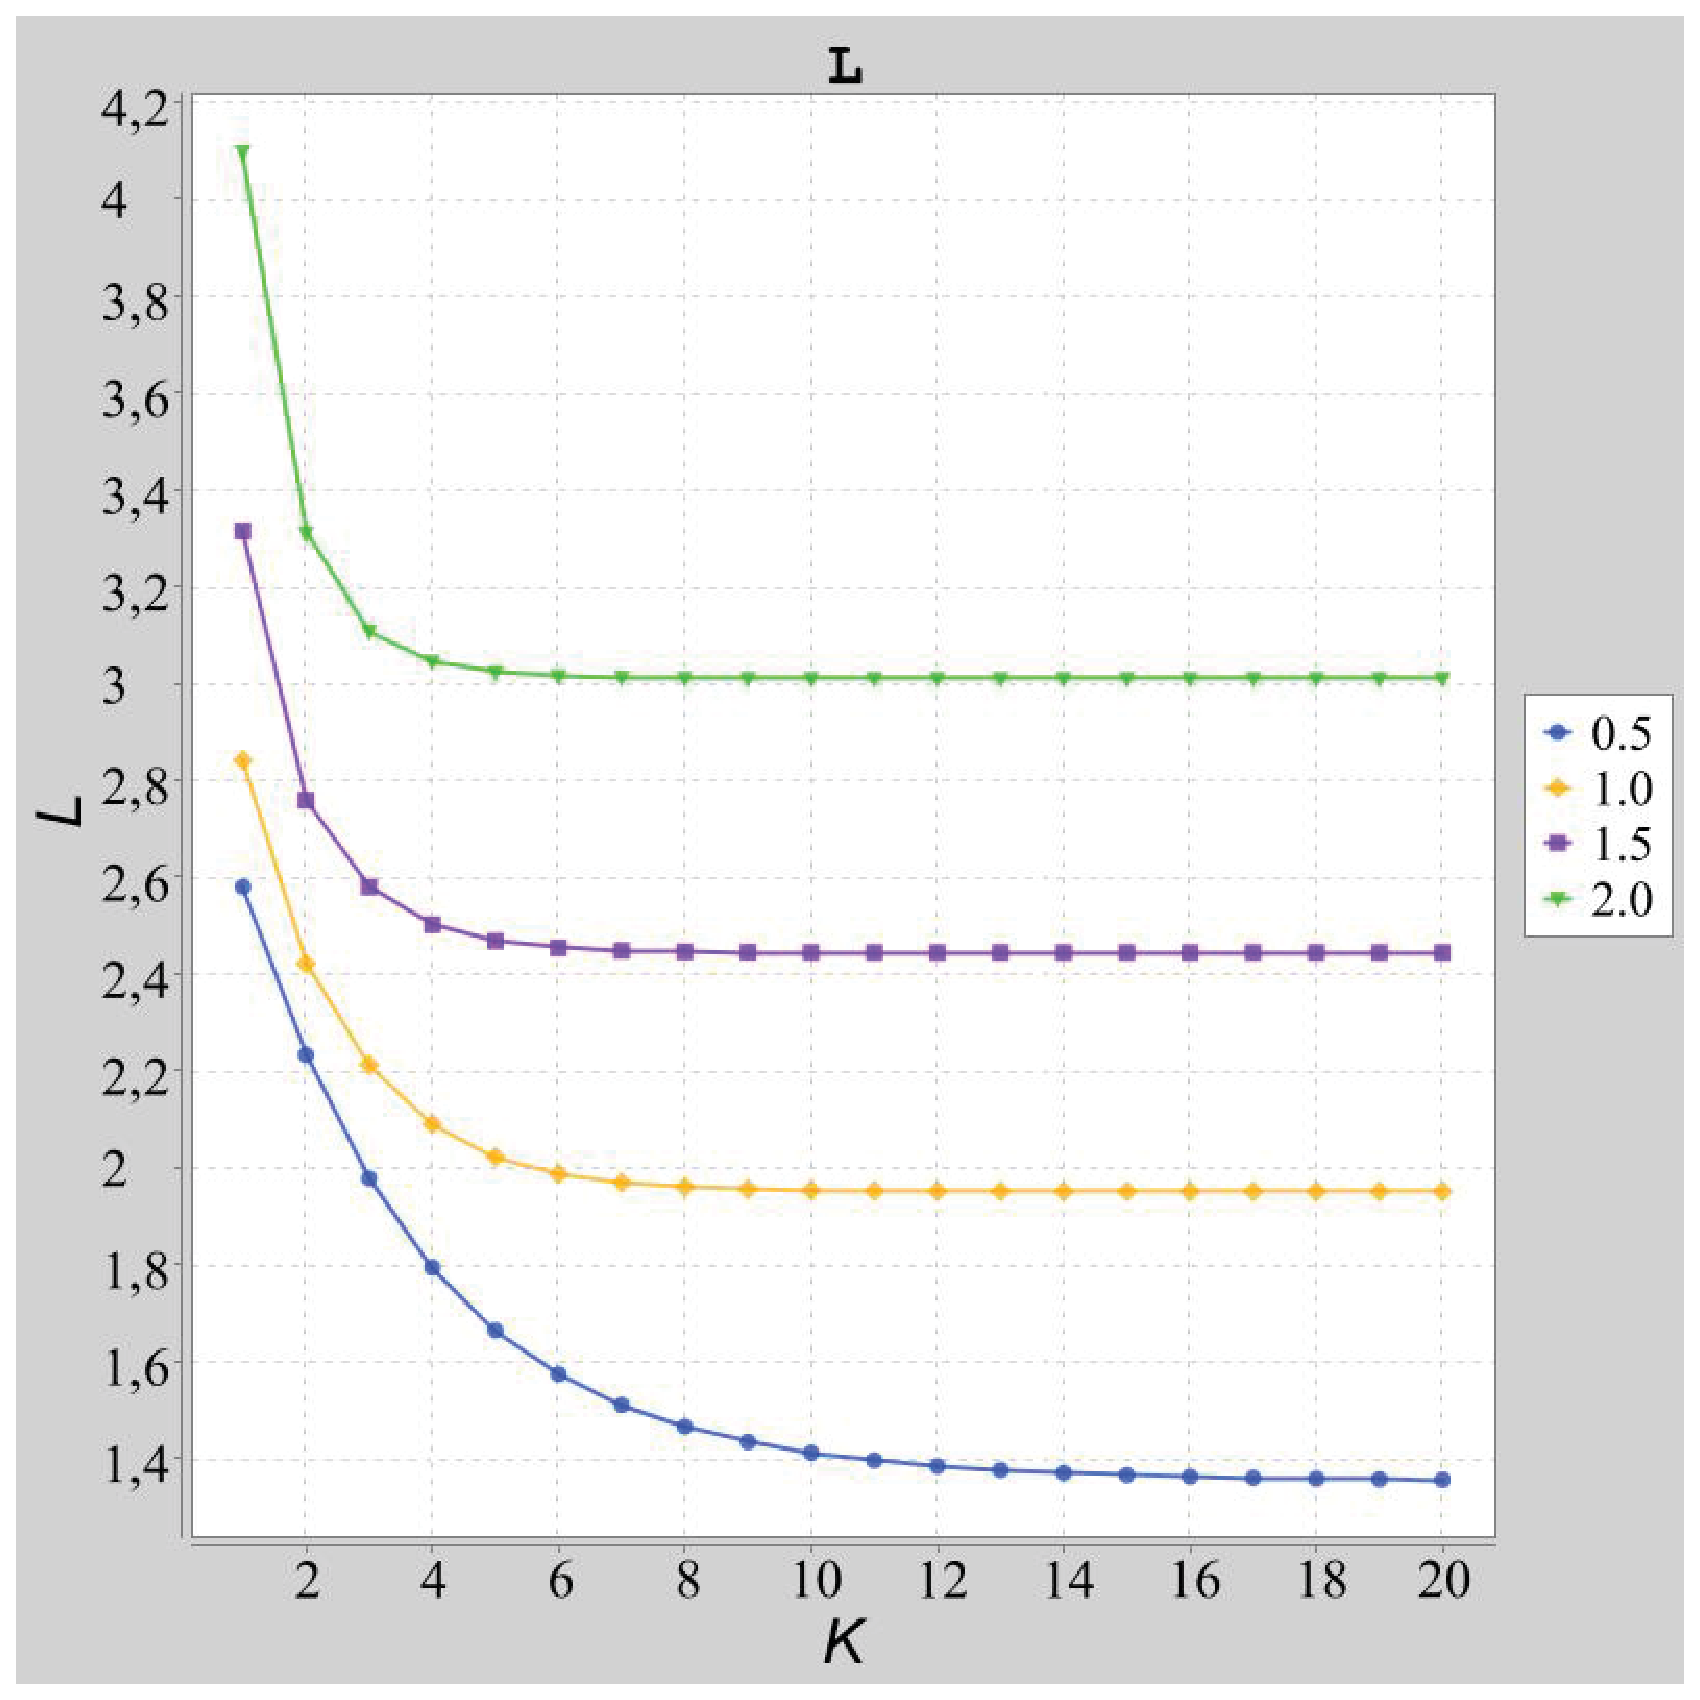
\includegraphics[width=1.0\linewidth]{Map/11.eps} \\ a)}
\end{minipage}
\hfill
\begin{minipage}[h]{0.49\linewidth}
\center{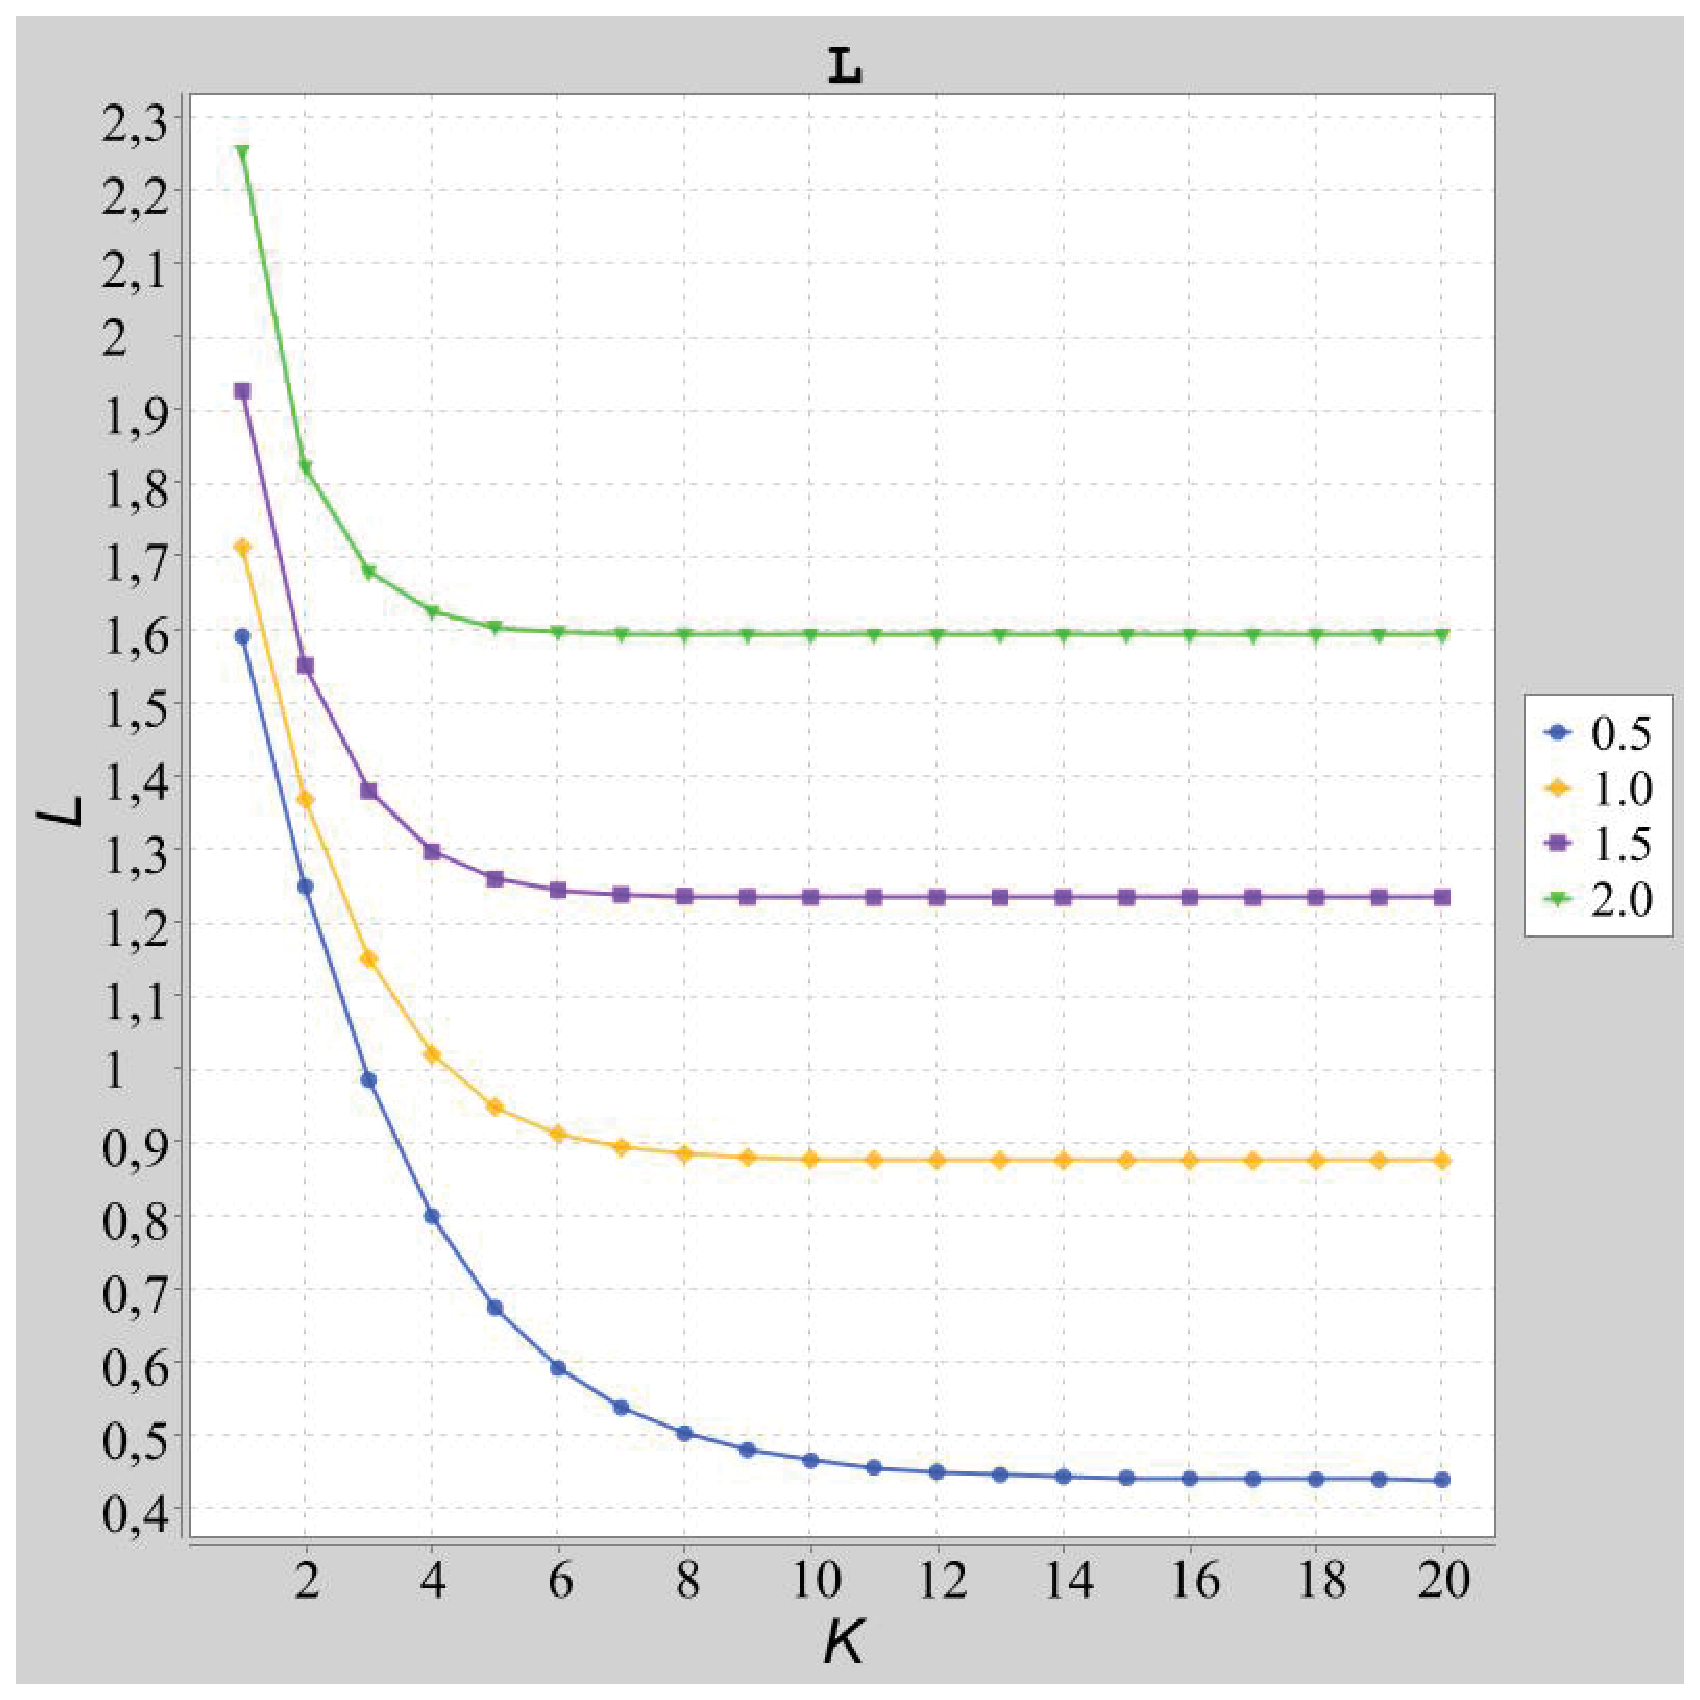
\includegraphics[width=1.0\linewidth]{st/21} \\ b)}
\end{minipage}
\caption{Dependence of the average number of customers in the system at service completion moments on the capacity $K$ of the stock
in cases of the $MAP$ (a) and stationary Poisson arrival process (b)}
%\label{ris:image1}
\end{figure}

\begin{figure}[h]
\begin{minipage}[h]{0.49\linewidth}
\center{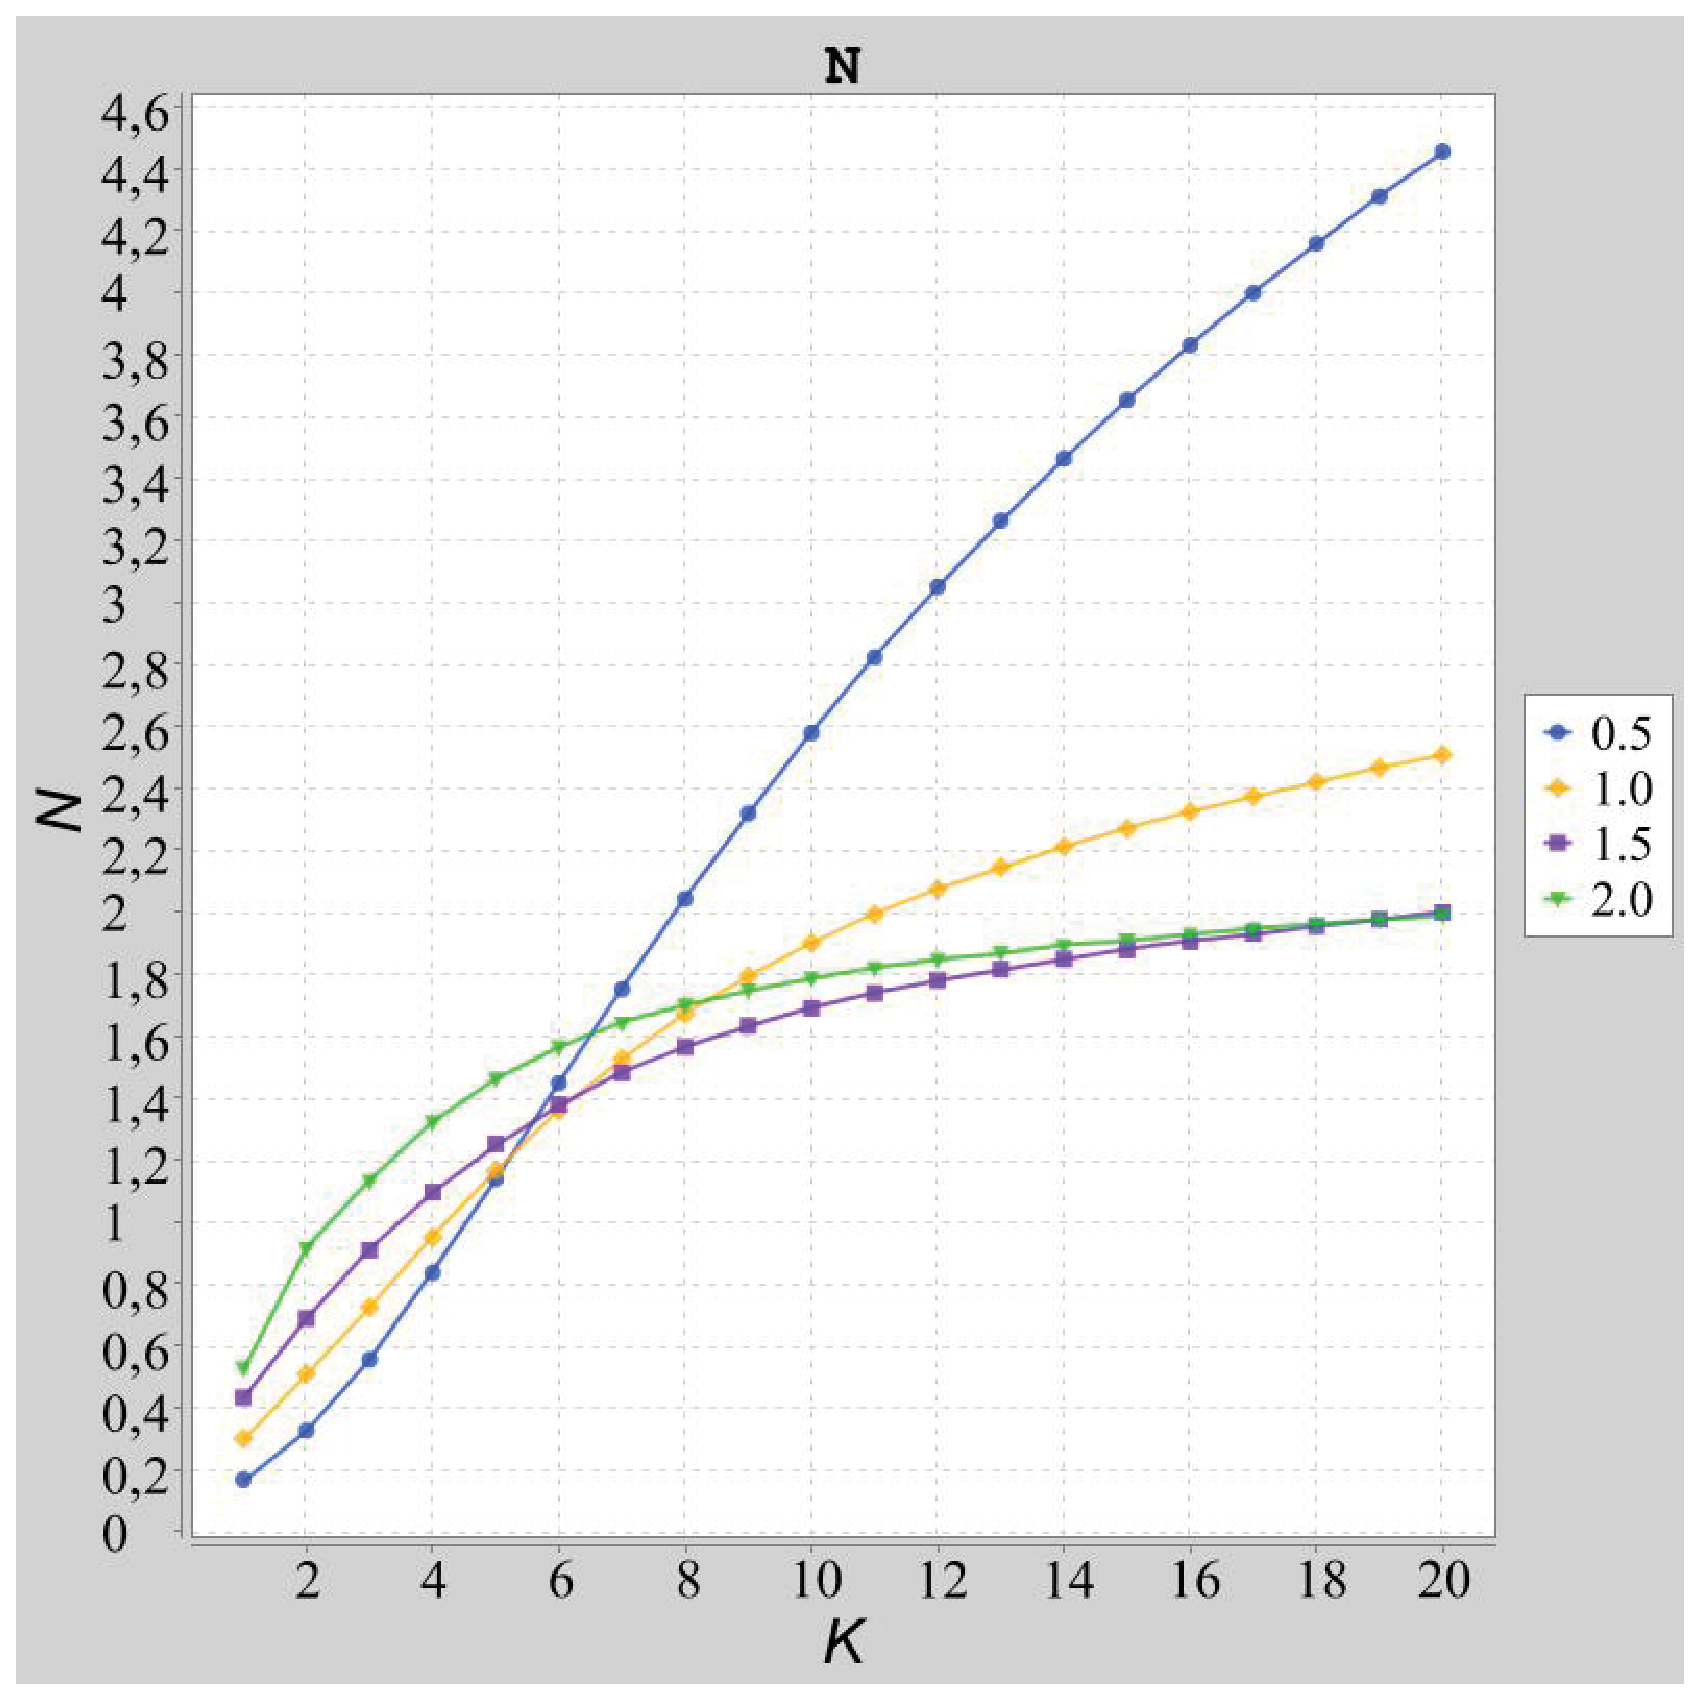
\includegraphics[width=1.0\linewidth]{Map/12.eps} \\ a)}
\end{minipage}
\hfill
\begin{minipage}[h]{0.49\linewidth}
\center{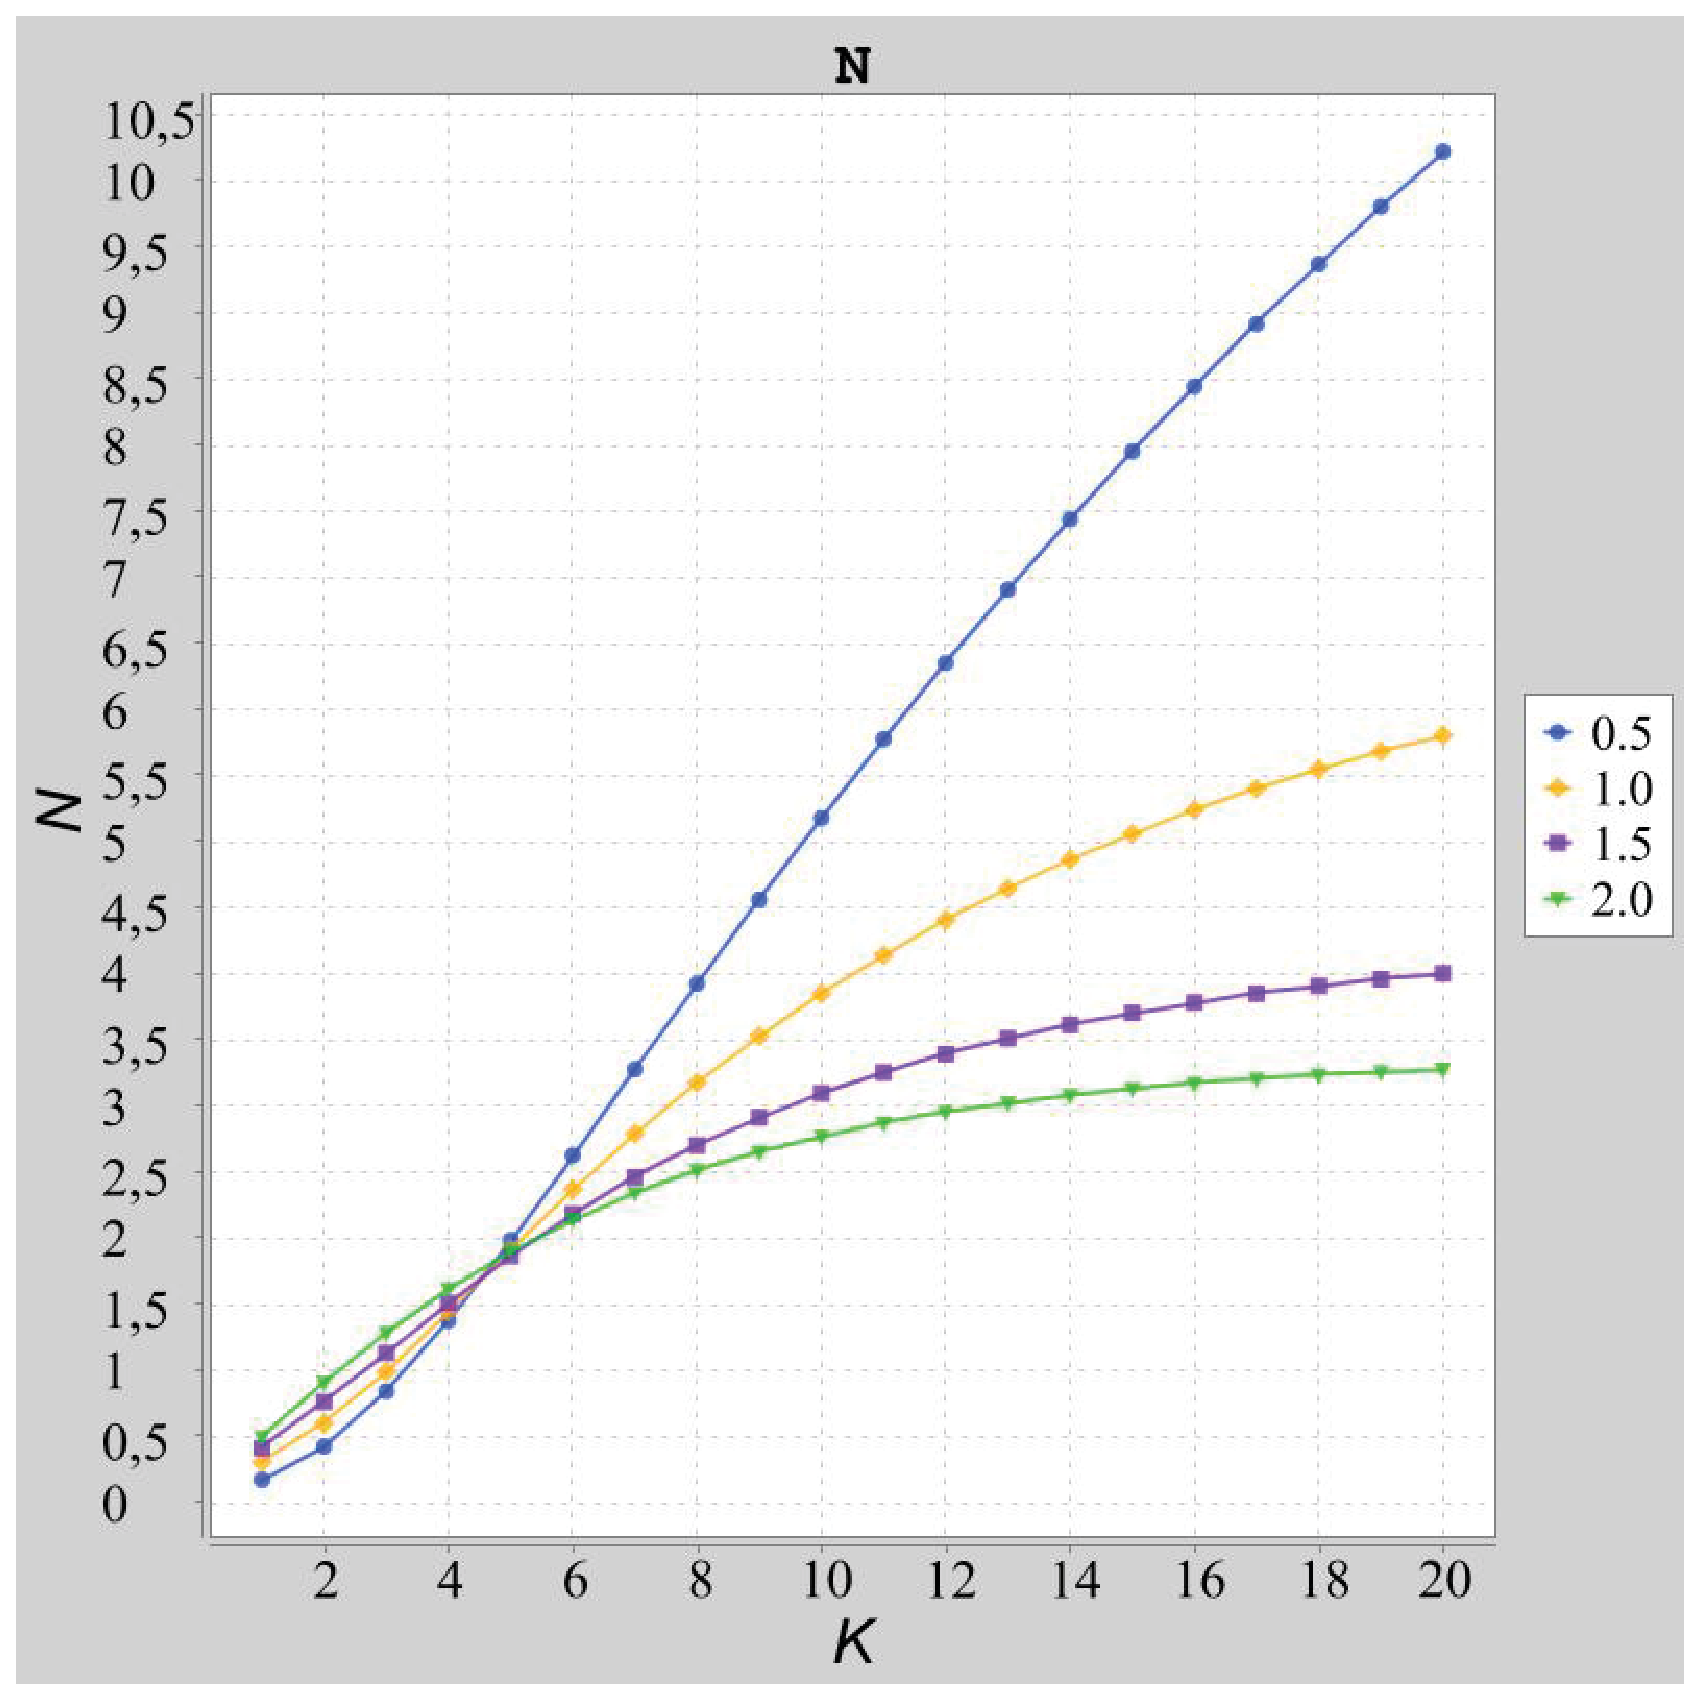
\includegraphics[width=1.0\linewidth]{st/22} \\ b)}
\end{minipage}
\caption{Dependence of the average number of energy units  at service completion moments on the capacity $K$ of the stock
in cases of the $MAP$ (a) and stationary Poisson arrival process (b)}
%\label{ris:image1}
\end{figure}


\begin{figure}[h]
\begin{minipage}[h]{0.49\linewidth}
\center{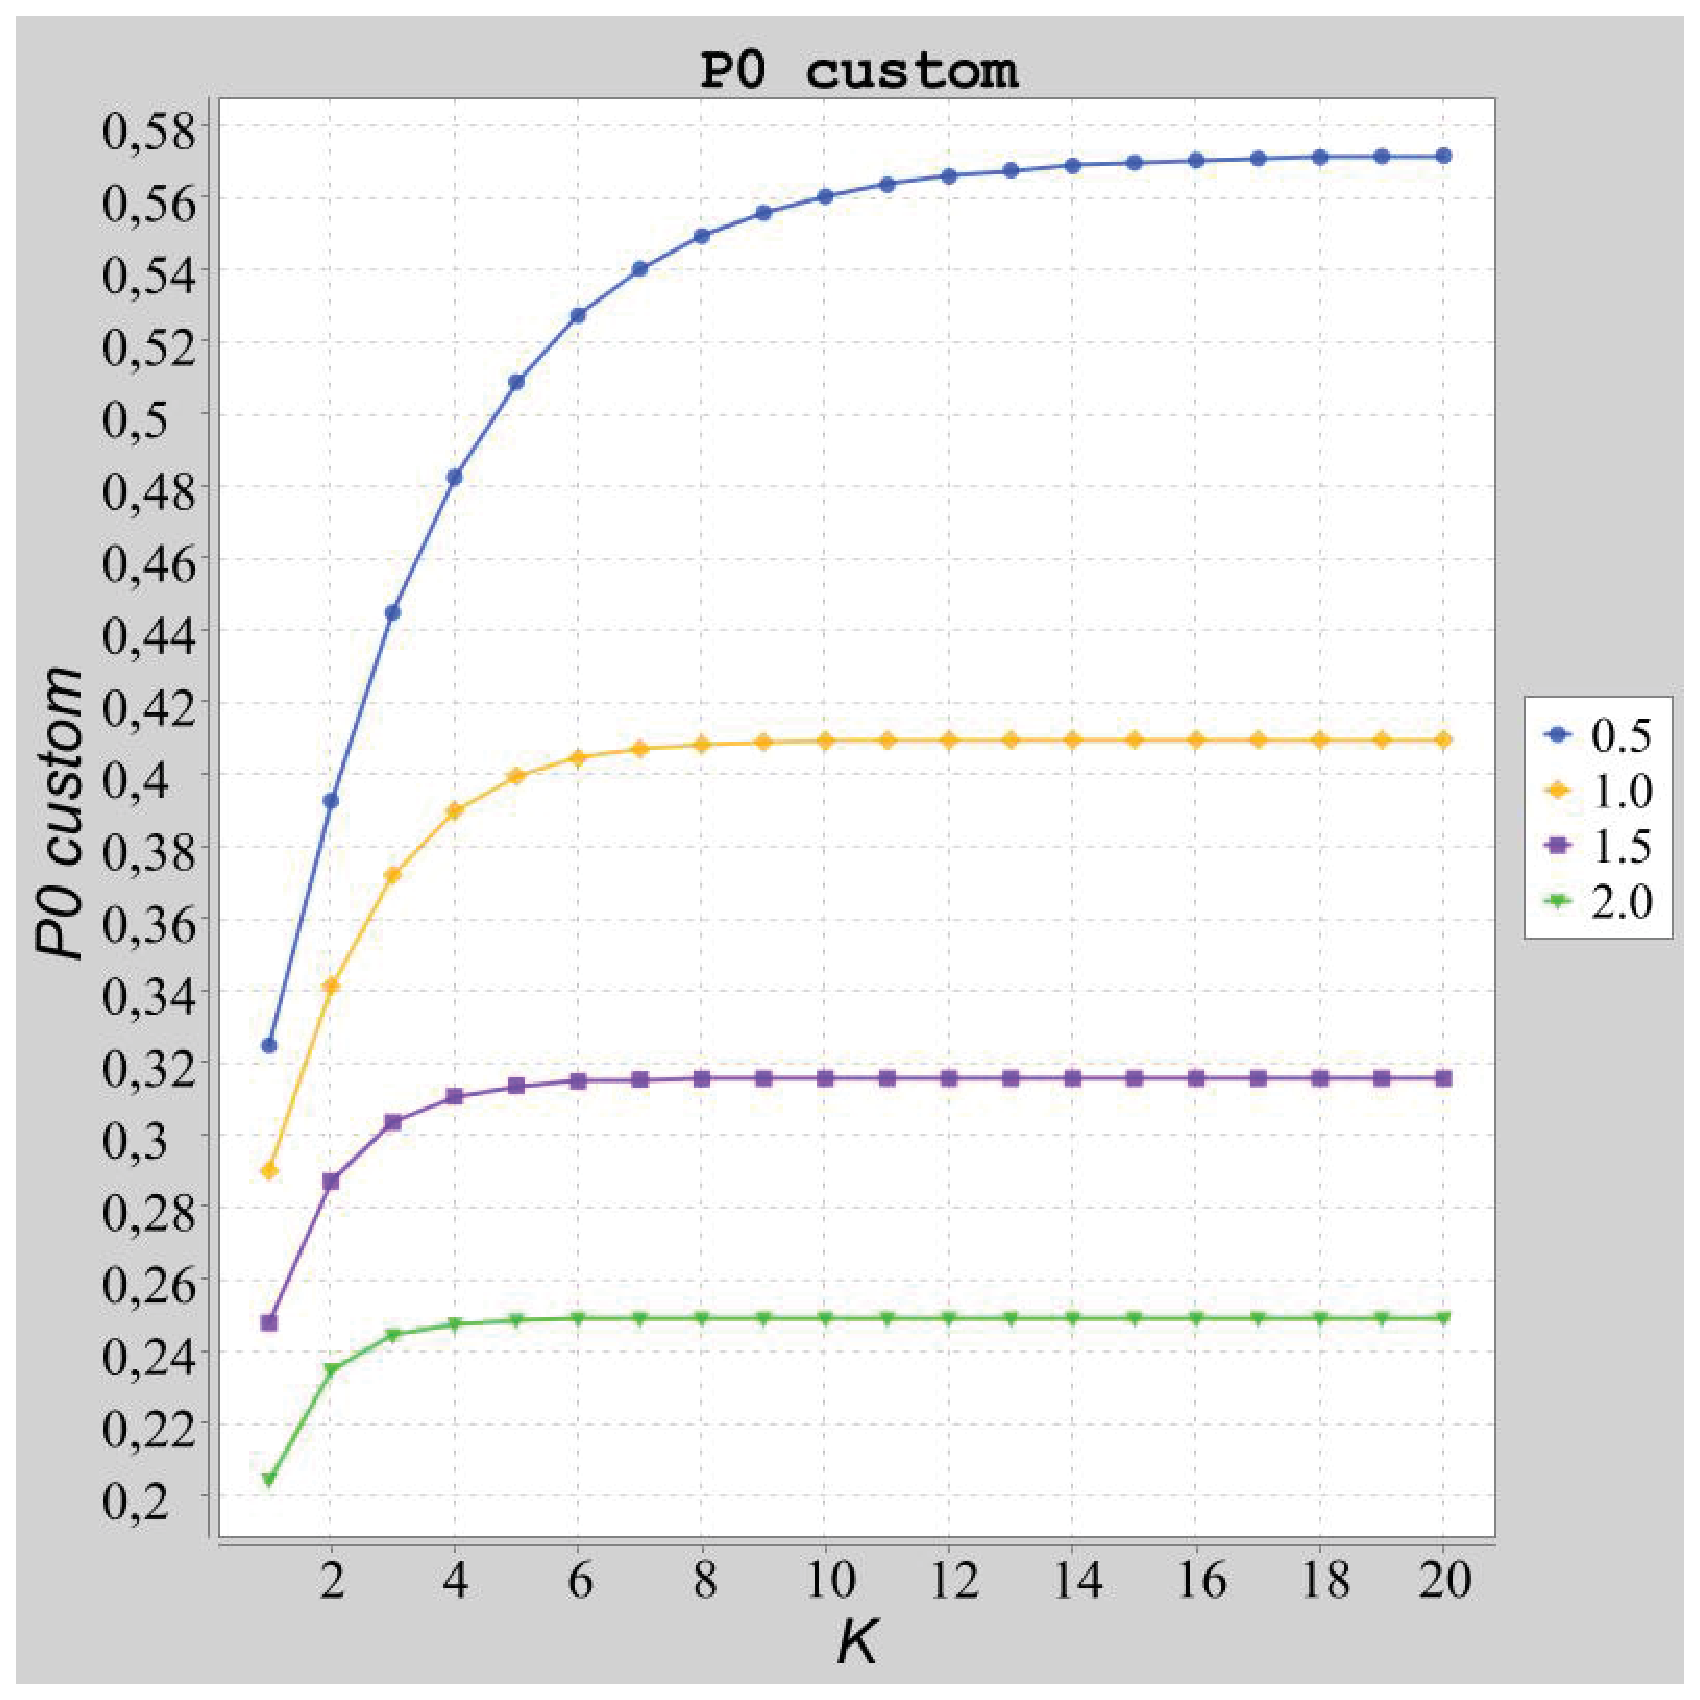
\includegraphics[width=1.0\linewidth]{Map/13.eps} \\ a)}
\end{minipage}
\hfill
\begin{minipage}[h]{0.49\linewidth}
\center{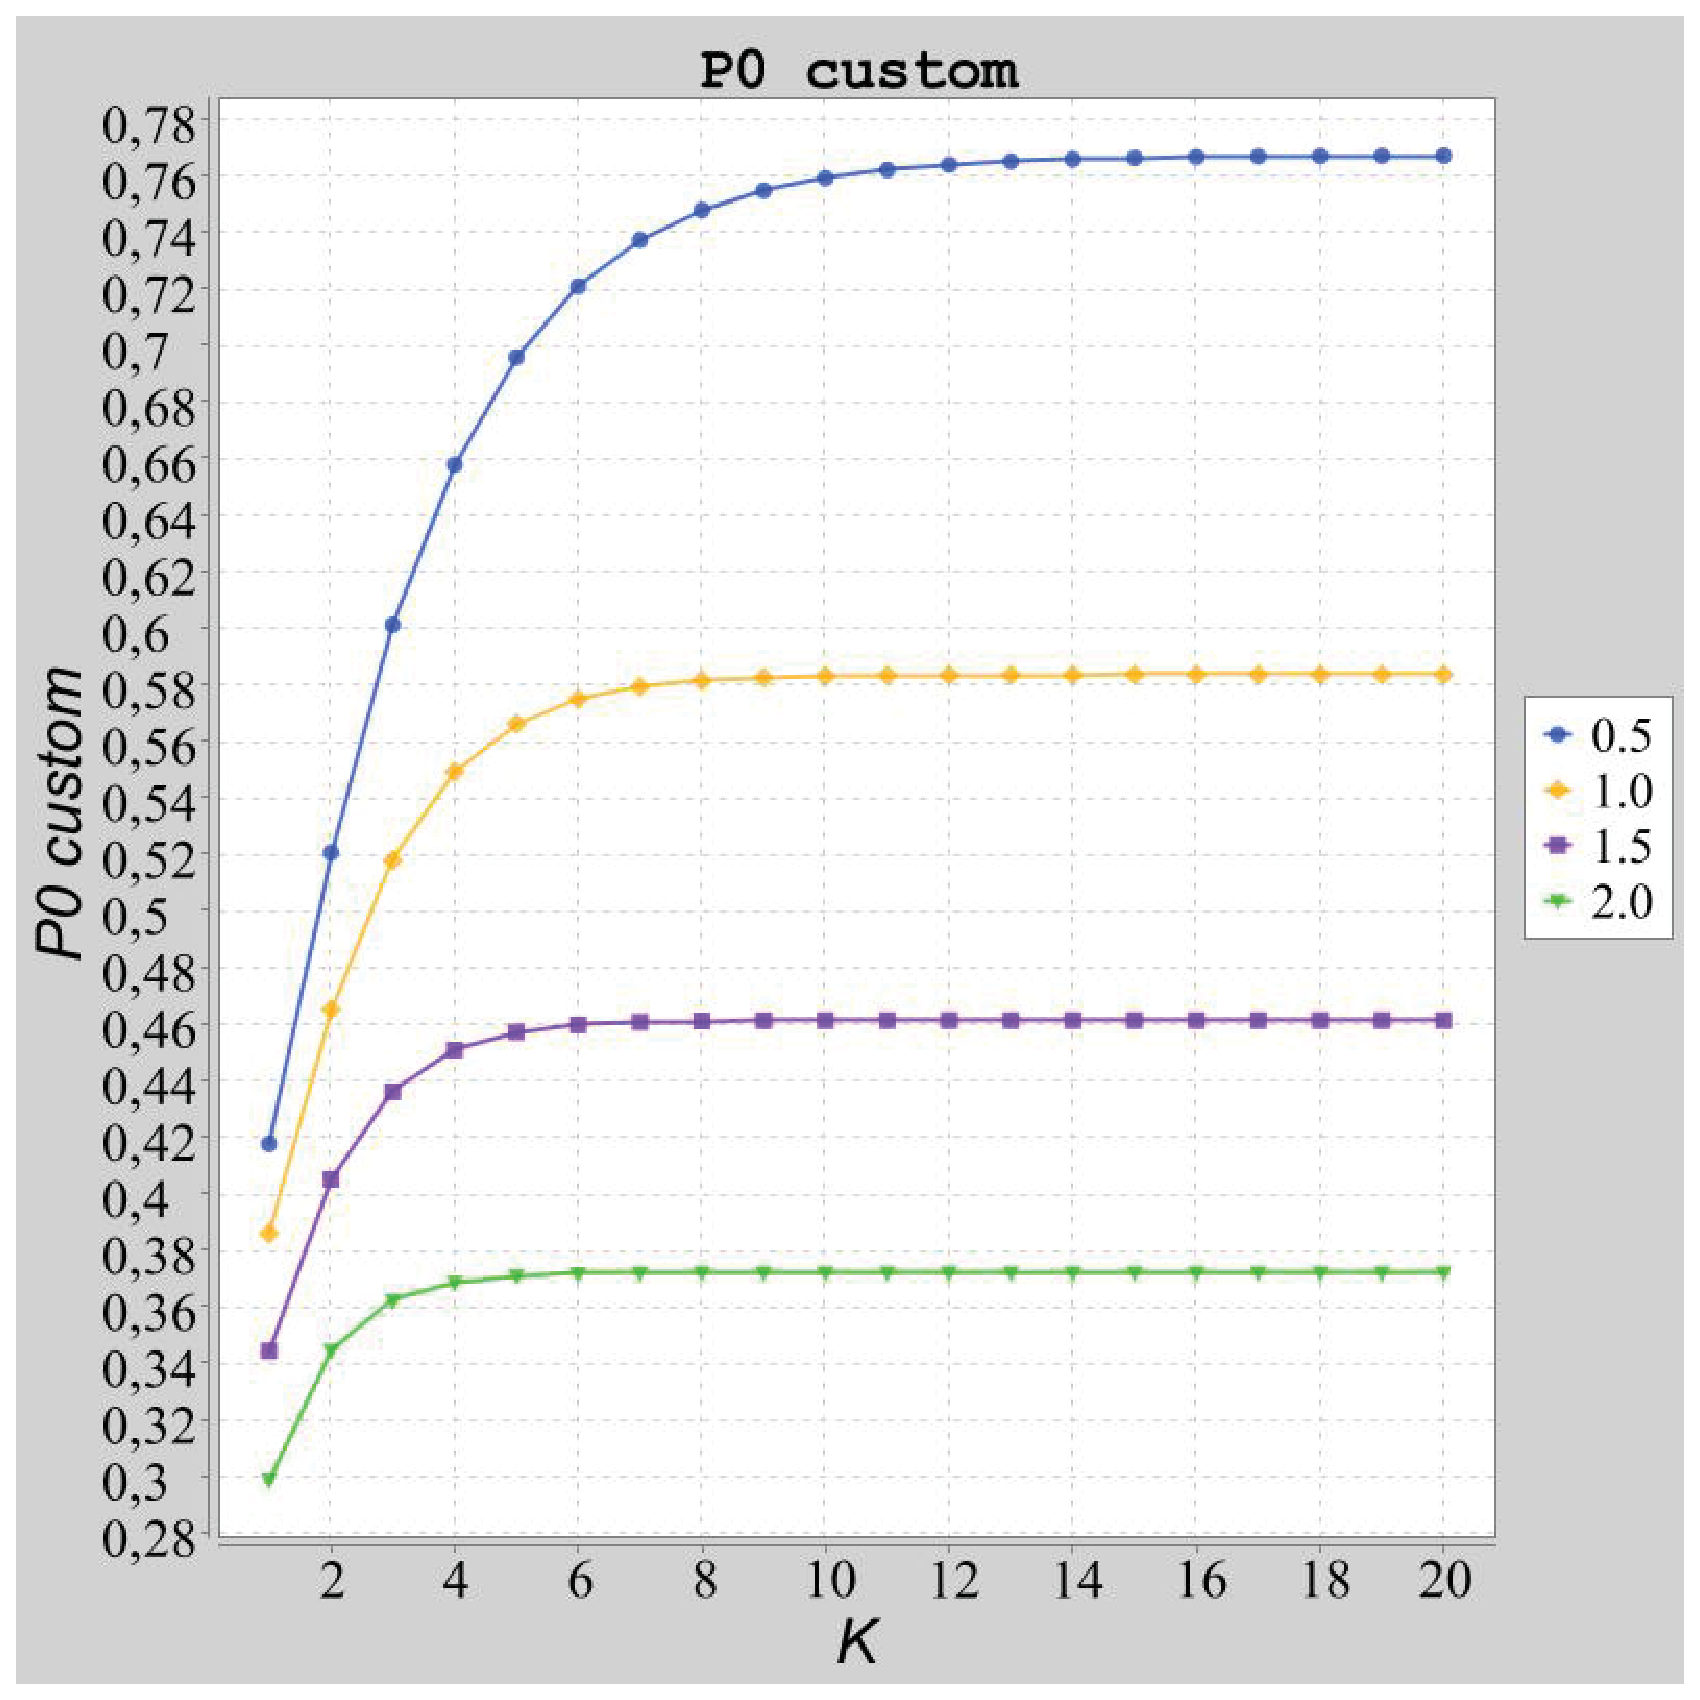
\includegraphics[width=1.0\linewidth]{st/23} \\ b)}
\end{minipage}
\caption{Dependence of the probability that there is no customer in the system at service completion moments on the capacity $K$ of the stock
in cases of the $MAP$ (a) and stationary Poisson arrival process (b)}
%\label{ris:image1}
\end{figure}

\begin{figure}[h]
\begin{minipage}[h]{0.49\linewidth}
\center{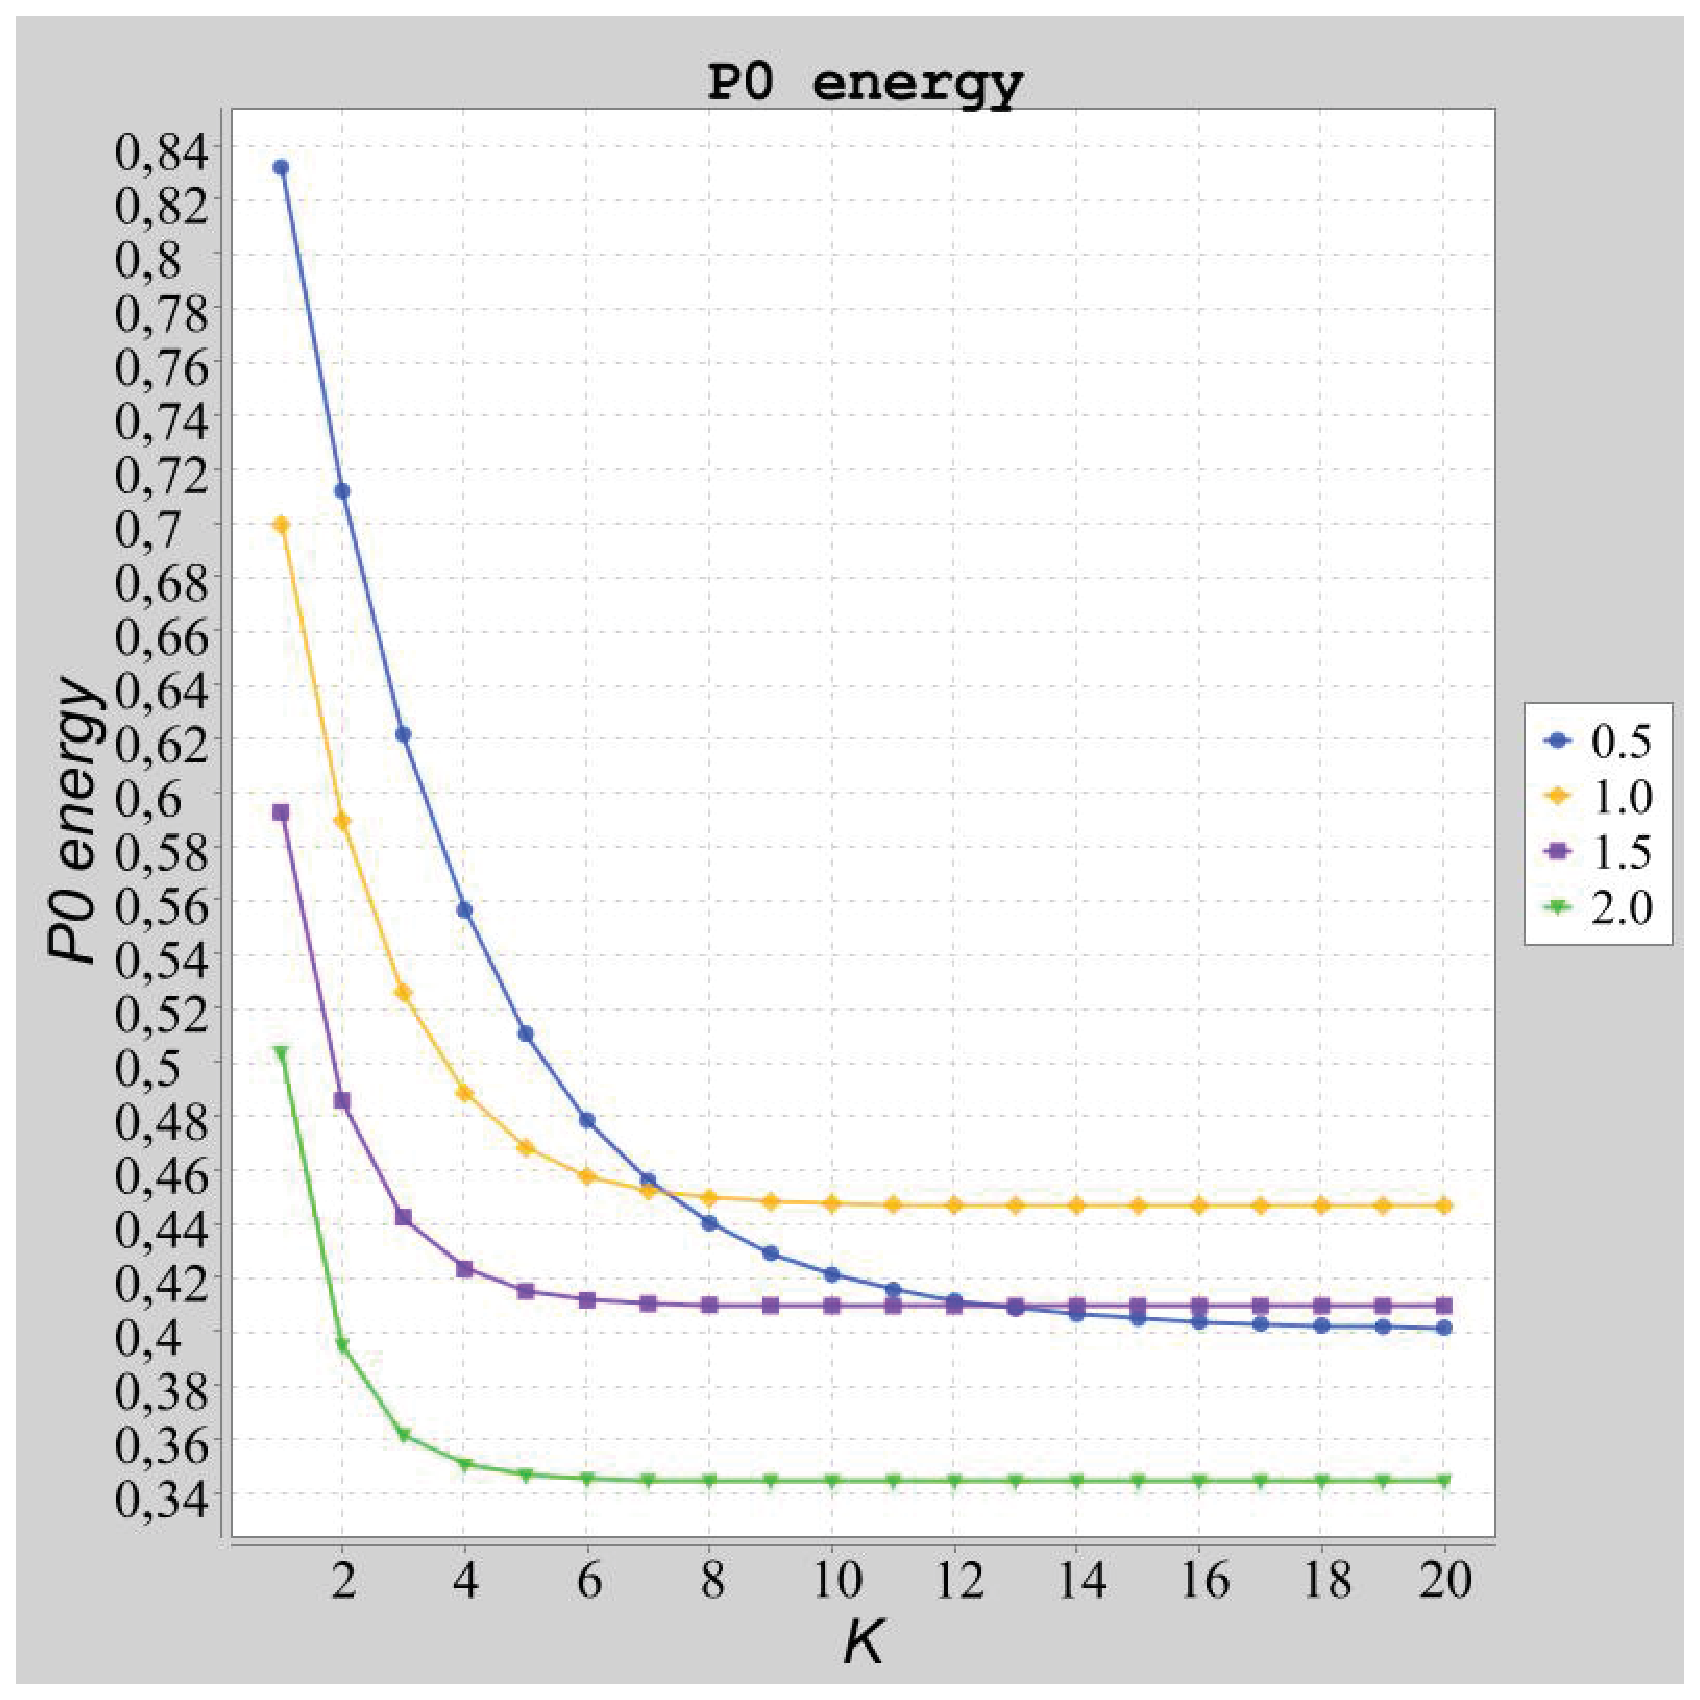
\includegraphics[width=1.0\linewidth]{Map/14.eps} \\ a)}
\end{minipage}
\hfill
\begin{minipage}[h]{0.49\linewidth}
\center{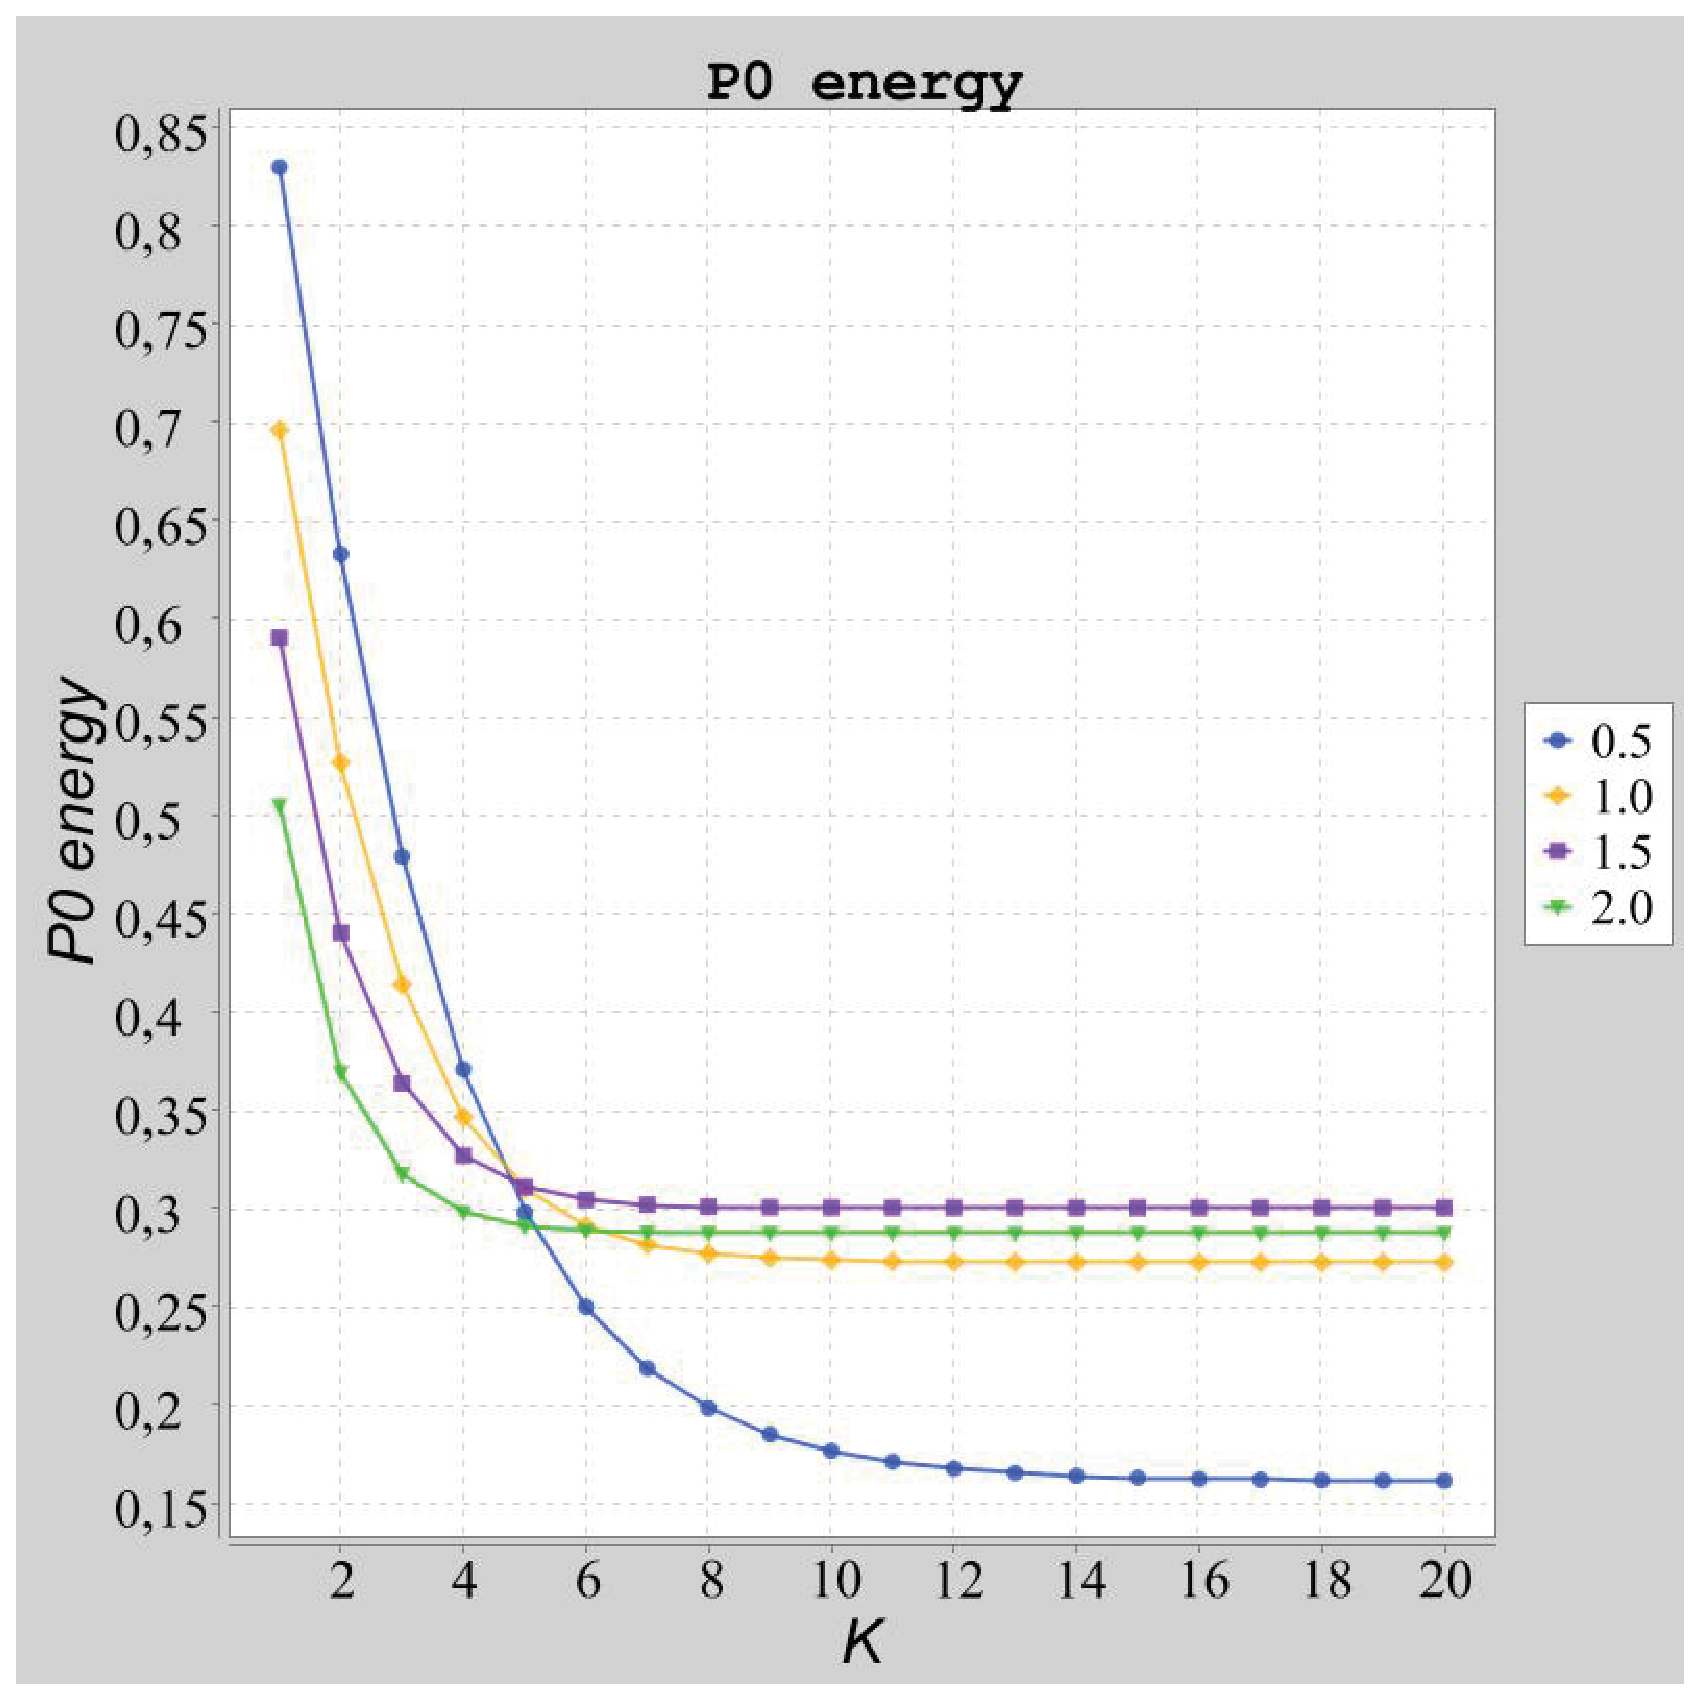
\includegraphics[width=1.0\linewidth]{st/24} \\ b)}
\end{minipage}
\caption{Dependence of the probability that there is no energy in the system at service completion moments on the capacity $K$ of the stock
in cases of the $MAP$ (a) and stationary Poisson arrival process (b)}
%\label{ris:image1}
\end{figure}


\begin{figure}[h]
\begin{minipage}[h]{0.49\linewidth}
\center{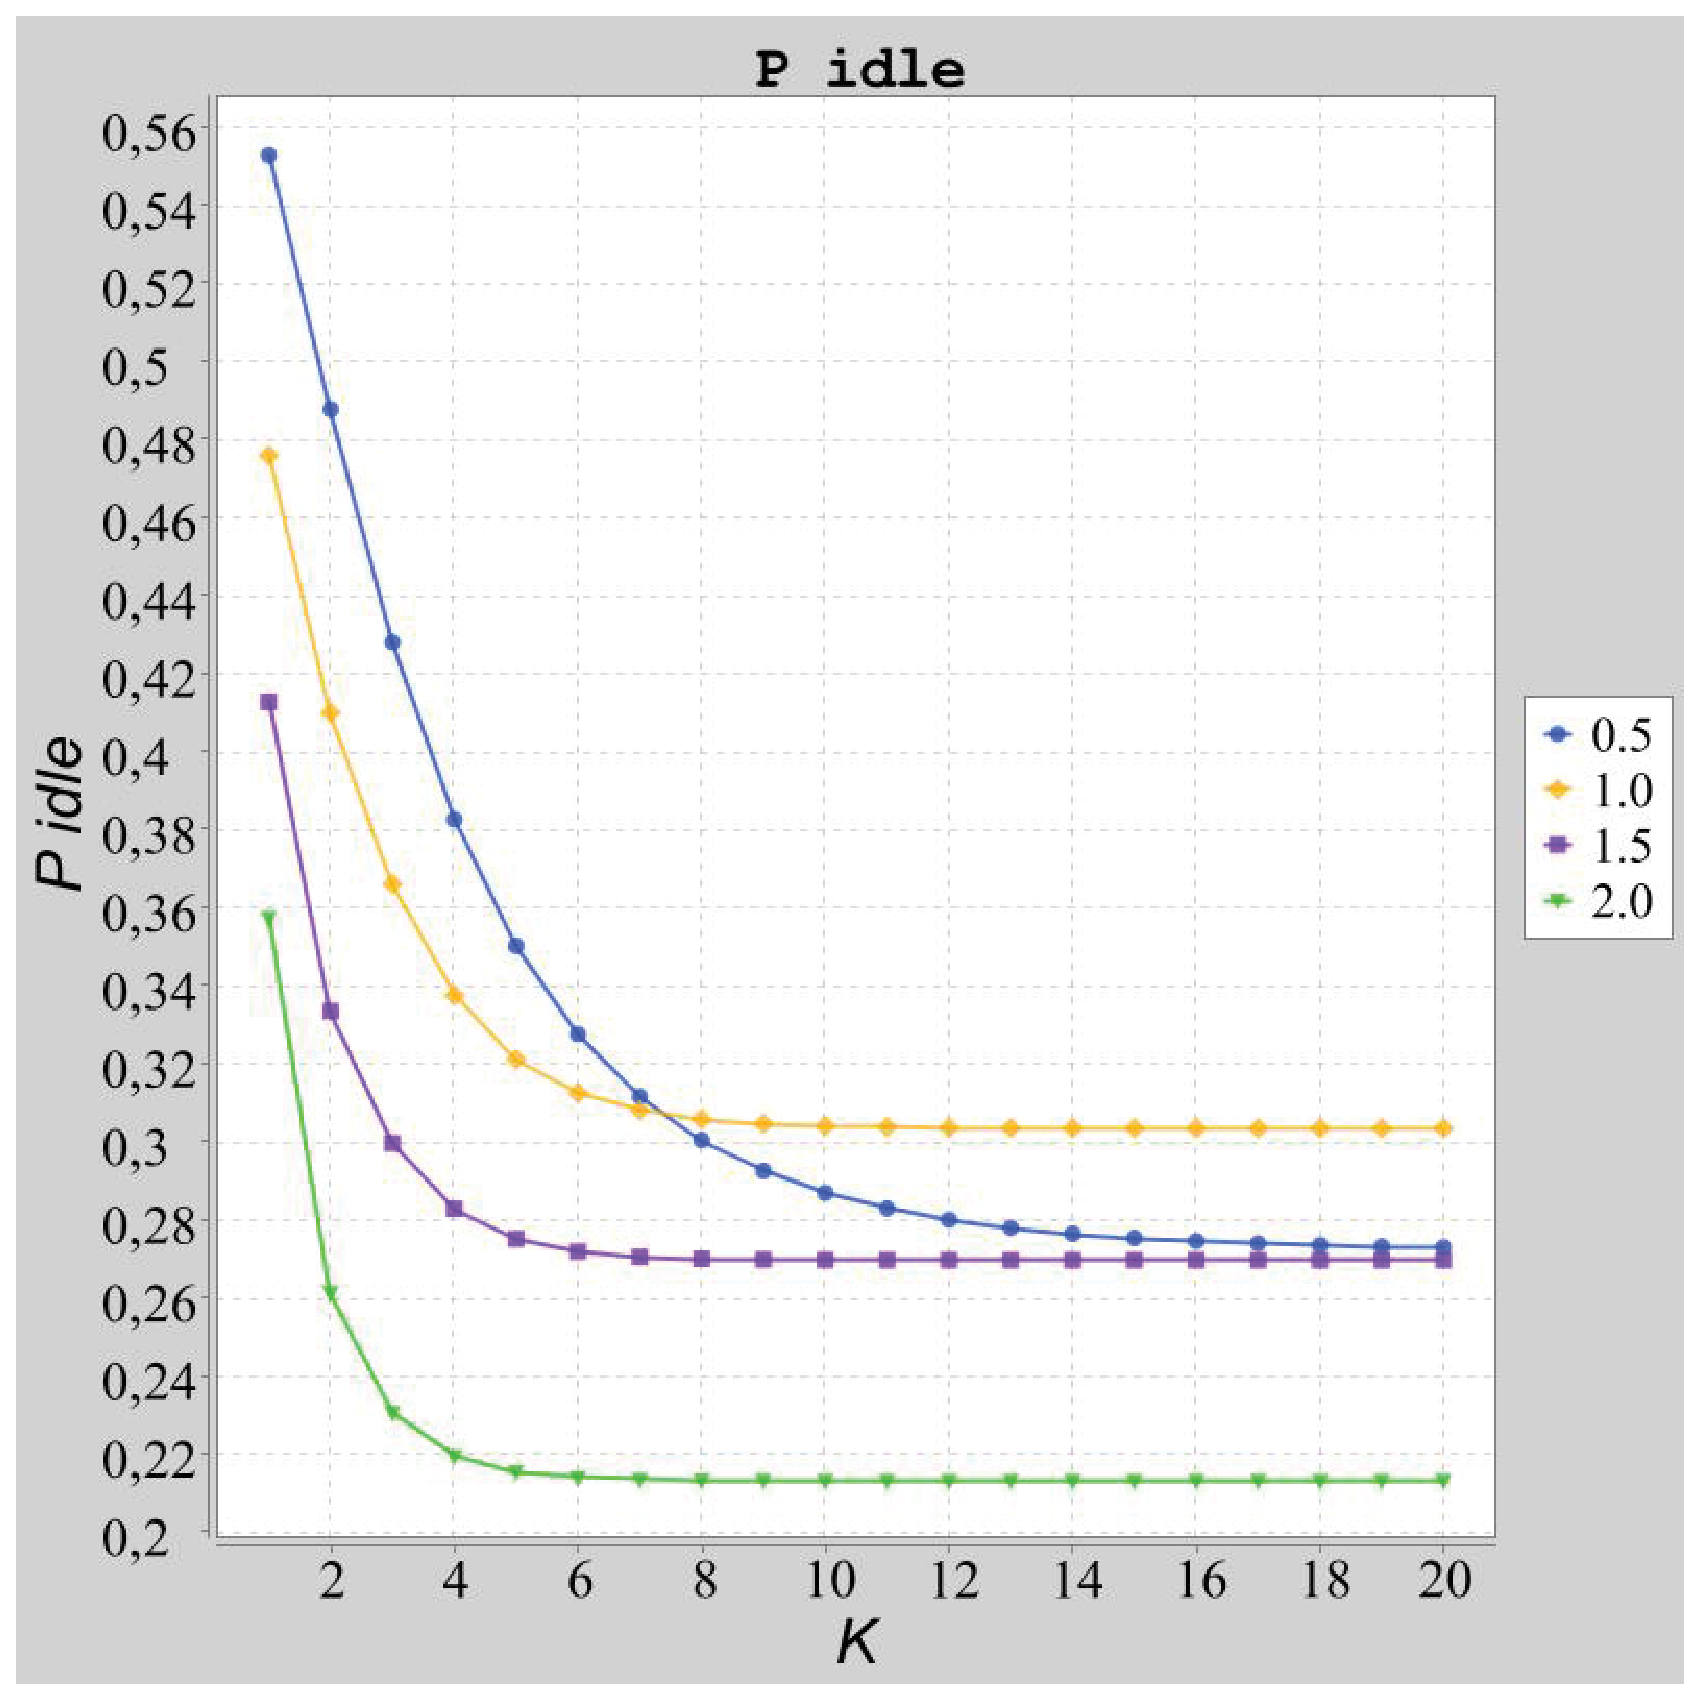
\includegraphics[width=1.0\linewidth]{Map/15.eps} \\ a)}
\end{minipage}
\hfill
\begin{minipage}[h]{0.49\linewidth}
\center{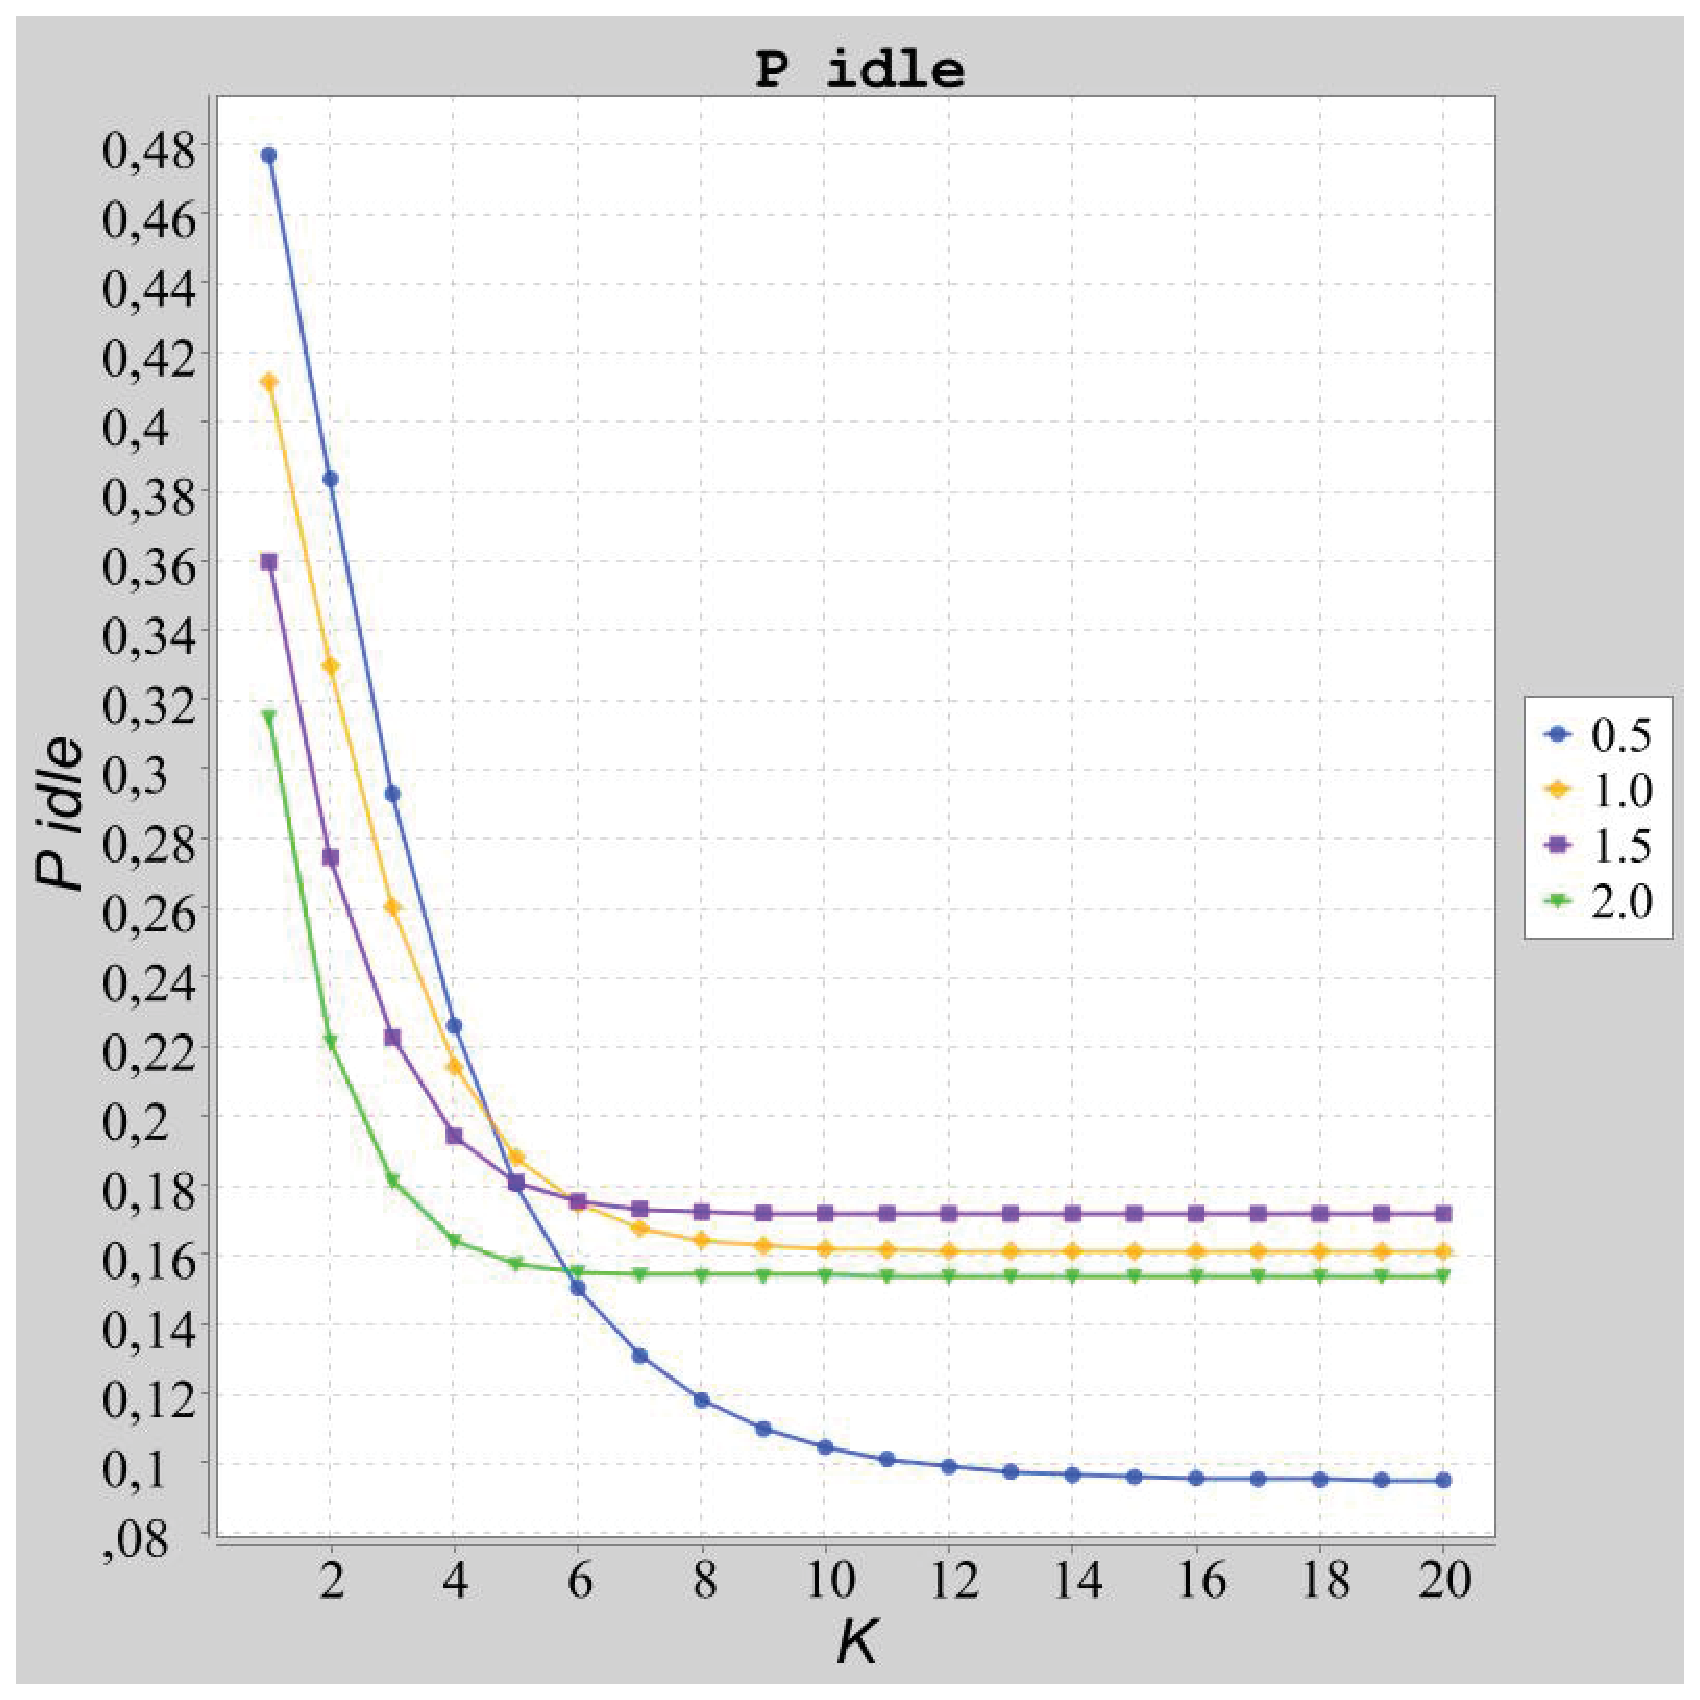
\includegraphics[width=1.0\linewidth]{st/25} \\ b)}
\end{minipage}
\caption{Dependence of the probability that there the server cannot start service due to the lack of energy in the system at service completion moments on the capacity $K$ of the stock
in cases of the $MAP$ (a) and stationary Poisson arrival process (b)}
%\label{ris:image1}
\end{figure}



% ---- Bibliography ----
%
% BibTeX users should specify bibliography style 'splncs04'.
% References will then be sorted and formatted in the correct style.
%
% \bibliographystyle{splncs04}
% \bibliography{mybibliography}
%
\begin{thebibliography}{8}

\bibitem{a}
A. Arafa, T. Tong, M. Fu, S. Ulukus and W. Chen,   Delay Minimal Policies in Energy Harvesting Communication Systems, IEEE Transactions on Communications 2018, DOI 10.1109/TCOMM.2018.2805357.

\bibitem{b1}
 A. A. Babayo,  M. H. Anisi,  I.  Ali,  A Review on energy management schemes in energy harvesting wireless sensor networks // Renewable and Sustainable Energy Reviews. vol.  76, pp. 1176-1184, 2017.

 \bibitem{b2}
 J.H. Baek, O. Dudina, C.S. Kim,   Queueing System with Heterogeneous Impatient Customers and Consumable Additional Items //     Applied Mathematics and Computer Science. vol. 27, No 2, pp. 367-384, 2017.



\bibitem{chak}
Chakravarthy S.R. The batch Markovian arrival process: a
review and future work, in: A. Krishnamoorthy, N. Raju, V. Ramaswami (Eds.), {Advances in Probability Theory and Stochastic
Processes},   Notable Publications Inc., New Jersey, 2001, pp. 21-29.

\bibitem{cinlar}
Cinlar E. Introduction to stochastic processes. Courier Corporation, 2013.

 \bibitem{cuy}
 E. De Cuypere,  K. De Turck, and D. Fiems, A queueing model of an energy harvesting sensor node with data buffering, Telecommunication Systems vol. 67, pp.  281-295, 2018.

 \bibitem{d1}
 S.A. Dudin,  M.H. Lee,  Analysis of single-server queue with phase-type service and energy harvesting. Mathematical Problems in Engineering.  vol. 2016, ID592794, pp. 1-16, 2016.

 \bibitem{d2}
 A. Dudin,    O. Dudina, Analysis of the $MAP/PH/1$ service system with repeat calls and energy audit // Automatic Control and Computer Science.  vol. 45, no 5, pp. 277-285, 2015.

 \bibitem{d3}
 A.N. Dudin, M.H. Lee, S.A. Dudin,  Optimization of Service Strategy in Queueing System with Energy Harvesting and Customers Impatience // Applied Mathematics and Computer Science.  vol. 26, no 2, pp. 367-378, 2016.

 \bibitem{d4}
 A. Dudin,   S. Dudin, O. Dudina, C.S. Kim, Analysis of  a wireless sensor node with varying rates of energy harvesting and consumption // Lecture Notes in Computer Science. V. 10684. 2017. P. 172-182.

\bibitem{dkv}
 Dudin A. N., Klimenok V.I., Vishnevsky V.M.   The theory of queuing systems with correlated flows. Springer. 2019.

 \bibitem{g1}
  E. Gelenbe, Synchronising energy harvesting and data packets
in a wireless sensor, Energies, vol. 8, no. 1, pp. 356-369, 2015.

 \bibitem{g2}
  E.Gelenbe, A sensor node with energy harvesting. ACM SIGMETRICS Performance Evaluation Review, vol. 42, no. 2, pp.37-39, 2014.

\bibitem{graham}
 Graham, A. Kronecker products and matrix calculus with
applications, Courier Dover Publications, 2018.

\bibitem{kim1}
C.S. Kim, A. Dudin,   S. Dudin, O. Dudina,    Performance Evaluation of a Wireless Sensor Node With Energy Harvesting and Varying Conditions of Operation // Proceedings of IEEE International Communication Conference.  pp.1-6, 2017.

\bibitem{kim2}
C.S. Kim, S.  Dudin   A. Dudin, K. Samouylov       Multi-threshold control by a single-server queuing model with a service rate depending on the amount of harvested energy, Performance Evaluation. 2018.   Vol. 127-128. P. 1-20.

\bibitem{kr1} A. Krishnamoorthy, B. Lakshmy,  and  R. Manikandan,  A survey on inventory models with positive service time,  Opsearch, vol. 48(2), pp.153-169, 2011.

\bibitem{kr2}
A. Krishnamoorthy,  D. Shajin, and  B. Lakshmy,  On a queueing-inventory with reservation, cancellation, common life time and retrial, Annals of Operations Research, vol. 247(1), pp.365-389, 2016.

\bibitem{luk}
   Lucantoni, D.M.  New results on the single server queue with a
batch Markovian arrival process, Communications in
Statistics-Stochastic Models. 7  (1991) 1-46.

\bibitem{neuts1989}
Neuts M.F.     Structured Stochastic Matrices of $M/G/1$ Type and
Their Applications.  Marcel Dekker. New York. 1989.

\bibitem{p}
K. Patil, K. De Turck, D. Fiems,
A two-queue model for optimising the value of information in energy-harvesting sensor networks,
Performance Evaluation, vol. 119, pp. 27-42,  2018.

\bibitem{s1}
 V. Sharma, U. Mukherji, V. Joseph, and S. Gupta, Optimal energy management policies for energy harvesting sensor
nodes, IEEE Transactions on Wireless Communications, vol. 9, no. 4, pp. 1326-1336, 2010.

\bibitem{s2}
H.H.R. Sherazi, L. A. Grieco,  G. Boggia, A Comprehensive Review on Energy Harvesting MAC Protocols in WSNs: Challenges and Tradeoffs, Ad Hoc Networks, vol. 71, pp. 117-134, 2018.

\bibitem{t1}
L. Tan, S. Tang,  Energy harvesting wireless sensor node with temporal death: Novel models and analyses // IEEE/ACM Transactions on Networking. vol. 25(2), pp. 896-909, 2017.

\bibitem{t2}
K. Tutuncuoglu and A. Yener, Optimum transmission policies for battery limited energy harvesting nodes, IEEE Transactions
on Wireless Communications, vol. 11, no. 3, pp. 1180-1189, 2012.

\bibitem{u}
S. Ulukus,  A. Yener, E. Erkip,   O. Simeone,  M. Zorzi,  P. Grover, and K. Huang,   Energy harvesting wireless communications: A review of recent advances, IEEE Journal on Selected Areas in Communications, vol. 33, pp. 360-381,  2015.



\bibitem{vd}
 Vishnevskii V. M.,   Dudin A. N. Queueing Systems with Correlated Arrival Flows
and Their Applications to Modeling Telecommunication Networks, Automation and Remote Control, 2017, Vol. 78, No. 8, pp. 1361–1403.

\bibitem{y1}
J. Yang and S. Ulukus, Optimal packet scheduling in an energy
harvesting communication system,IEEE Transactions on Communications, vol. 60, no. 1, pp. 220-230, 2012.

\bibitem{y2}
J.Yang and S.Ulukus, Optimal packet scheduling in a multiple
access channel with energy harvesting transmitters, Journal of
Communications and Networks, vol. 14, pp. 140-150, 2012.






\end{thebibliography}


%\end{document}

{\bf Appendix A. Proof of Lemma 5.}



{\bf Proof.}
Using the notations introduced in Lemma 1, we have:
$$
C_{k,k'}^0=\int\limits_0^\infty e^{D_0t}\phi_{k'-k}(t)dt, \,\,0\leq k\leq k'\leq K-1,
$$
$$
C_{k,K}^0=\int\limits_0^\infty e^{D_0t}\hat{\phi}_{K-k}(t)dt, \,\,0\leq k\leq K.
$$


$$ C_{0,k'}^{(j)}(s)=\int\limits_0^\infty  P(j,t)\phi_0(t)dt ({\cal B}(s))_{0,k'}+
$$
$$
+\int\limits_0^\infty \int\limits_0^t e^{D_0x}\gamma e^{-\gamma x}dx
e^{D_0(t-x)}\sum\limits_{l=0}^{k'}{\phi}_l(t-x)D_1dt \Psi_{k'-l}(j-1,s)+
$$
$$
+\int\limits_0^\infty \int\limits_0^t e^{D_0x}\phi_0(x)D_1dx \sum\limits_{l=0}^{j-1}P(l,t-x)\gamma e^{-\gamma (t-x)}dt
\Psi_{k'}(j-l-1, s),
$$
$$
j\geq1, 0\leq k'\leq K-2,
$$


$$
 C_{0,K-1}^{(j)}(s)=\int\limits_0^\infty  P(j,t)\phi_0(t)dt ({\cal B}(s))_{0,K-1}+
 $$
 $$+
  \int\limits_0^\infty \int\limits_0^t e^{D_0x}\gamma e^{-\gamma x}dx
e^{D_0(t-x)}
[\sum\limits_{l=0}^{K-1}{\phi}_l(t-x)D_1dt  \Psi_k-l-1(j-1,s)dt+
$$
$$
+\sum\limits_{l=K}^\infty{\phi}_l(t-x)D_1dt \Psi_0(j-1,s)]+
$$
$$
+\int\limits_0^\infty \int\limits_0^t e^{D_0x}\phi_0(x)D_1dx \sum\limits_{l=0}^{j-1}P(l,t-x)\gamma e^{-\gamma (t-x)}dt
\Psi_{K-1}(j-l-1,s),
 j\geq1,
$$


$$
 C_{0,K}^{(j)}(s)=\int\limits_0^\infty \int\limits_0^t e^{D_0x}\gamma e^{-\gamma x}dx
e^{D_0(t-x)}[\sum\limits_{l=0}^{K-1}{\phi}_l(t-x)D_1dt
){\bar\Phi}_{K-l}(j-1,s))dt
+
$$
$$
+\sum\limits_{l=K}^{\infty}{\phi}_l(t-x)D_1dt
 \sum\limits_{l=1}^{\infty} {\bar\Phi}_1(j-1,s)]dt]+
$$
$$
+\int\limits_0^\infty \int\limits_0^t e^{D_0x}\phi_0(x)D_1dx \sum\limits_{l=0}^{j-1}P(l,t-x)\gamma e^{-\gamma (t-x)}dt
{\bar\Phi}_K(j-l-1, s)]dt,
 j\geq 1;
$$

$$
 C_{k,k'}^{(j)}(s)=
\int\limits_0^\infty e^{D_0t}\sum\limits_{l=0}^{k'-k+1}{\phi}_l(t)D_1dt \Psi_{k'-k-l+1}(j-1, s),\,
 k\geq1, k-1\leq k'\leq K-2, j\geq1.
$$

$$
 C_{k,K-1}^{(j)}(s)=
\int\limits_0^\infty e^{D_0t}[\sum\limits_{l=0}^{K-k}{\phi}_l(t)D_1dt
\Psi_{K-k-l}(j-1,s)+
\sum\limits_{l=K-k+1}^\infty{\phi}_l(t)D_1dt \Psi_0(j-1,s)],
$$
$$
 k\geq1,  j\geq1.
$$



$$
C_{k,K}^{(j)}(s)=\sum\limits_{l=0}^{K-k}
\int\limits_0^\infty e^{D_0t}{\phi}_l(t)D_1dt \sum\limits_{n=K-k-l+1}^\infty {\bar \Phi}_{K-k-l+1}(j-1, s)+
$$
$$
+\sum\limits_{l=K-k+1}^\infty
\int\limits_0^\infty e^{D_0t}{\phi}_l(t)D_1dt
 \sum\limits_{n=1}^\infty {\bar \Phi}_1(j-1,s), \,
j>0, k=\overline{1, K},
$$



$$
\Omega_{0,k'}^{(r)} (s)=\int\limits_0^\infty \sum\limits_{l=0}^{(r)} P(l,t)\gamma e^{-\gamma t}dt
\tilde{ \Phi}_{k'}(r,s),
k'=\overline{0,K-1}, r\geq 0,
$$

$$
\Omega_{0,K}^{(r)} (s)=\int\limits_0^\infty \sum\limits_{l=0}^{(r)} P(l,t)\gamma e^{-\gamma t}dt
{\bar \Phi}_K(r,s),
k'=\overline{K-2,K-1}, r\geq 0,
$$


$$
\Omega_{k,k'}^{(r)} (s)=\tilde{ \Phi}_{k'-k+1}(r,s),
 k=\overline{1,K}, k'=\overline{k-1,K-1},  r\geq 0,
$$

$$
\Omega_{k,K}^{(r)} (s)={\bar \Phi}_{K-k+1}(r,s),
 k=\overline{k-1,K},  r\geq 0.
$$



%\end{document}

{\bf Appendix B. Computation of the matrices $\tilde{\Phi}(n,k),\;
n\geq0,\, k=\overline{0,K}$}

These matrices are easily computed, e.g., when service time has phase type distribution. Let us illustrate computation of  the matrices $\tilde{\Phi}(n,k)$ in the case when  service time does not have phase type distribution. Namely, we consider the constant service time. In this case, the distribution function $B(t)$ has the form
%\end{document}
$$
B(t)=\left\{
\begin{array}{cc}
0, & \;t\leq b_1,\\
1, & \;t>b_1.
\end{array}
\right.
$$
and, therefore, we have
$$
\tilde{\Phi}(n,k) = \int\limits_{0}^{\infty} P(n,t)\varphi_{k}(t)(1-B(t))dt=\int\limits_{0}^{b_1} P(n,t)\varphi_{k}(t)dt.\eqno(16)
$$


 To calculate the integral in (16), we use the well-known uniformization procedure.

Denote  $h=\max\limits_{i=\overline{0,W}}(-D_0)_{ii}$.

Then the matrix  $P(n,t),\; n\ge 1,$ can be represented in the following form:
$$
P(n,t)=\sum_{j=0}^{\infty}e^{-h t}{(h
t)^j\over j!}K_n^{(j)},\; n\ge 0,  \eqno(17)
$$
where the matrices  $K_n^{(j)},\; n\ge 1, j\ge 0,$ are calculated by recursion

$$
K_0^{(0)}=I,\ K_n^{(0)}=O,\ n\ge 1,
$$ $$
K_0^{(j+1)}=K_0^{(j)}(I+h^{-1}D_0),
$$ $$
K_n^{(j+1)}=h^{-1}K_{n-1}^{(j)}D_1+K_n^{(j)}(I+h^{-1}D_0),\; n\ge 1,\; j\ge 0.
$$

Substituting  expression (17) for $P(n,t)$ and expression for $\varphi_{k}(t)$ in (16) and simplifying, we obtain the following relations:
$$
\tilde{\Phi}(n,k)=\sum\limits_{j=0}^\infty K_n^{(j)} \frac{h^j\gamma^k}{j!k!} \int\limits_{0}^{b_1} e^{-(h+\gamma)t}t^{j+k}dt=
$$
$$=\sum\limits_{j=0}^\infty K_n^{(j)} \frac{h^j\gamma^k}{j!k!} \biggl[ \frac{(j+k)!}{(h+\gamma)^{j+k+1}}-e^{-b_1(h+\gamma)}\sum\limits_{l=0}^{j+k}\frac{(j+k)!}{l!}
\frac{b_1^l}{(h+\gamma)^{j+k-l+1}}\biggr]=
$$
$$
=\sum\limits_{j=0}^\infty K_n^{(j)} \frac{h^j\gamma^k}{j!k!}\frac{(j+k)!}{(h+\gamma)^{j+k+1}}\biggl[ 1-e^{-b_1(h+\gamma)}\sum\limits_{l=0}^{j+k}\frac{[b_1(h+\gamma)]^l}{l!}
\biggr]=
$$
$$=\frac{1}{(h+\gamma) k!}
\biggl(\frac{\gamma}{h+\gamma}\biggr)^k
\sum\limits_{j=0}^\infty K_n^{(j)}\frac{(j+k)!}{j!}
\biggl({\frac{h}{h+\gamma}}\biggr)^j \biggl[ 1-e^{-b_1(h+\gamma)}\sum\limits_{l=0}^{j+k}\frac{[b_1(h+\gamma)]^l}{l!}
\biggr].
$$
Thus, the matrix $\tilde{\Phi}(n,k)$ is equal to
$$=\frac{1}{(h+\gamma) k!}
\biggl(\frac{\gamma}{h+\gamma}\biggr)^k
\sum\limits_{j=0}^\infty K_n^{(j)}\frac{(j+k)!}{j!}
\biggl({\frac{h}{h+\gamma}}\biggr)^j \biggl[ 1-e^{-b_1(h+\gamma)}\sum\limits_{l=0}^{j+k}\frac{[b_1(h+\gamma)]^l}{l!}
\biggr].
$$



\end{document}
